\documentclass[fontsize=12pt,a4paper,final]{scrartcl}[2003/01/01]
\usepackage[ngerman]{babel} 
\usepackage[T1]{fontenc}
\usepackage[utf8]{inputenc} 
\usepackage{float}
\usepackage{listings}
\usepackage{color}
\usepackage{hyperref}
\usepackage{tabularx}
\usepackage[toc,page]{appendix}
\setlength{\parindent}{0pt}
                           
\lstset{ 
   language=Java, 
   breaklines=true,             
   tabsize=4,
   numbers=left,
   frame=single
} 

\title{Robotik Dokumentation - Team Robofreunde n.V.}
\author{Lohr, Schramm, Stumpf, Weber, Wurth}

\date{\today}

%Bilder scalen, wenn größer als Seite
\usepackage[final]{graphicx}
\makeatletter
\def\ScaleIfNeeded{%
	\ifdim\Gin@nat@width>\linewidth
		\linewidth
	\else
		\Gin@nat@width
	\fi
}
\makeatother

\begin{document}
Es handelt sich hier nur um einen Vorschlag für die Struktur des Dokuments. Das Ding erhebt keinen Anspruch auf Vollständigkeit, sondern ist das Ergebnis von maximal 15 Minuten \glqq Fuck, wir müssen den Shit fertig machen, ich fang mal an lol\grqq. Bevor wir dann wirklich anfangen aufzuteilen, wer was schreibt (abseits der offensichtlichen Stellen), sollten wir die Struktur des Dokuments \textbf{zusammen} durchgehen und finalisieren. Btw, ich hab keinen Plan von Latex, sollte ich also gegen irgendwelche Konventionen verstoßen haben würde es mich nicht wundern... Hoffe aber es passt einigermaßen. Manu


\maketitle
\tableofcontents

\section{Einleitung}\label{se:Einleitung}
\textit{Verfasser: Stumpf}\\
\\
Die Lehrveranstaltung Robotik im SS-2015 hatte die Programmierung des NAO -- eines humanoiden Roboters von Aldebaran -- als übergreifendes Thema. Diesem sollten für Fussball notwendige Bewegungsabläufe und Taktiken beigebracht werden. Aufgrund des großen Andrangs könnten sich nicht alle Teilnehmer mit dem einzigen zur Verfügung stehenden NAO Modell beschäftigen. Die Gruppe wurde also in ein Hardware und 2 Simulationsteams aufgeteilt.\\
\\
Die vorgegebene Simulationumgebung war die auf Simspark basierende RoboCup 3D-Soccer Simulation League.\\
Das vorgegebene Ziel unserer beiden Simulationsteams war es, je eine eigene Mannschaft aufs Feld zu bringen und diese am Ende gegeneinander antreten zu lassen.\\
\\
RoboCup ist eine Fussball-Liga humanoider Roboter. Die Teams mehrerer Länder treten gegeneinander an um ein bestes Team zu ermitteln.\\
\\
In der RoboCup Soccer Simulation League werden die Spiele simuliert. Die Roboter werden durch virtuelle Instanzen ersetzt, die über definierte Schnittstellen auf den Server verbunden und gesteuert werden können.\\
\\
Es gibt eine 2D und eine 3D Version. Für uns war insbesondere die 3D Version interessant, weil NAO hier das aktuelle Robotermodell ist. Anforderungen und Regeln der 3D Version sind vergleichbar mit dem echten RoboCup.\\
\\
Da die Schnittstellen zum Server auf sehr niedriger Ebene definiert sind - Bewegung von Gelenken - ist es für den Zeitraum der Lehrveranstaltung zu aufwändig, einen virtuellen Roboter komplett selbstständig zu entwickeln. Es gibt allerdings einige Frameworks, auf denen die eigene Arbeit aufgebaut werden kann.

\section{Anforderungen}
\textbf{-> TODO: Freddy???}
\textit{Was waren die allgemeinen Anforderungen?}
\section{Zeitplan}
\textit{Verfasser: Stumpf, Schramm, Wurth}\\
\\
Die folgende Timeline soll ein Überblick über den Verlauf der Lehrveranstaltung geben und insbesondere die Frage \textit{\glqq Wann wurde was gemacht?\grqq} beantworten.

\begin{figure}[H]
	\centering
	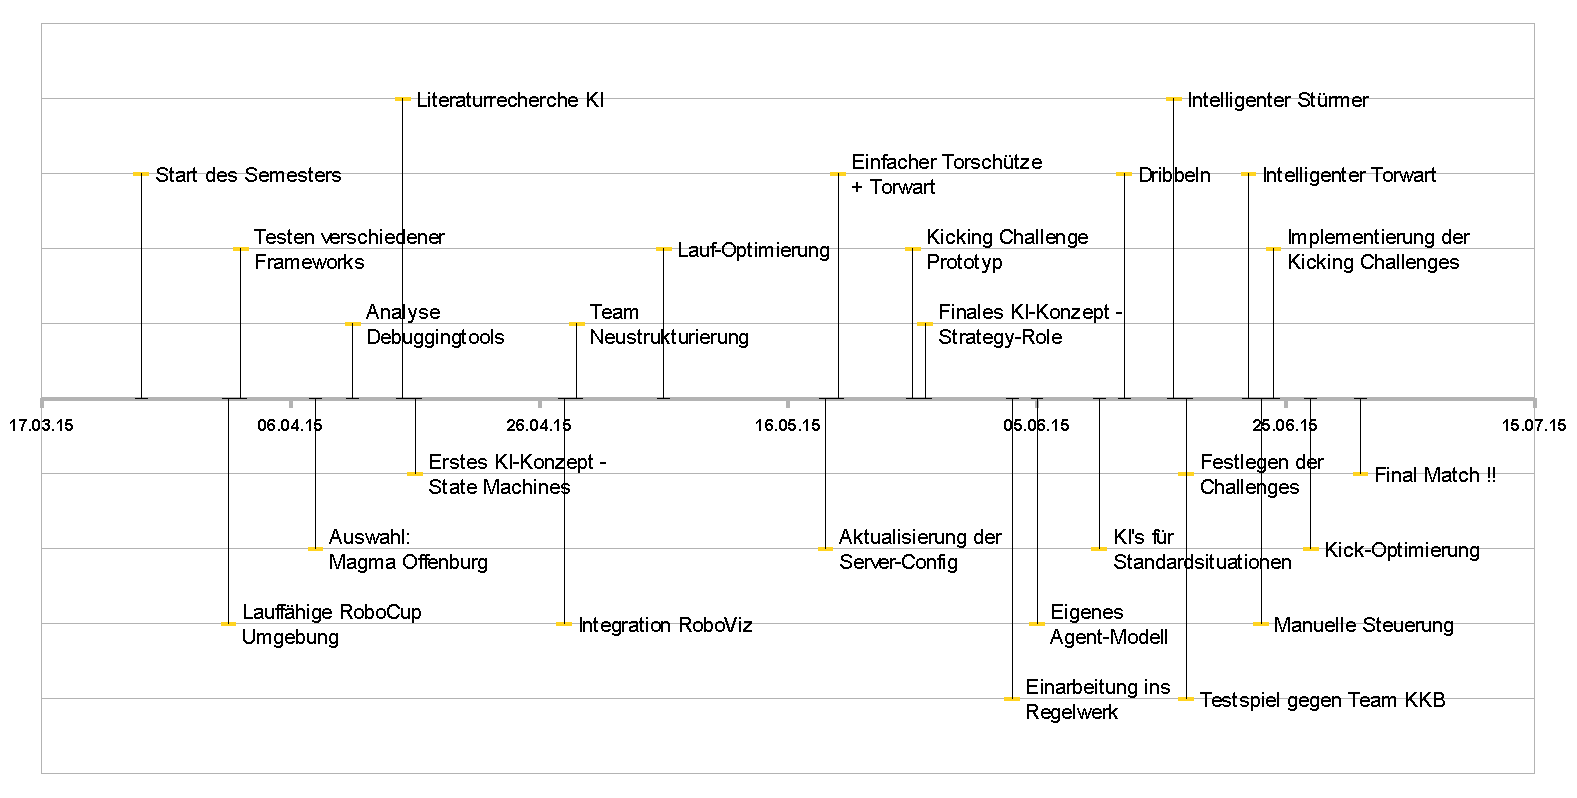
\includegraphics[width=\textwidth]{Grafiken/Timeline_cropped}
	\caption{Team Robofreunde - Timeline}
	\label{fig:Timeline}
\end{figure}

\section{RoboCup Soccer Simulation League}
\textit{Verfasser: Stumpf}\\
\\
Simspark ist die Engine, auf der der die RoboCup Soccer Simulation League aufgebaut ist. Es wird beschrieben als generisches Simulationssystem für mehrere Agents und ist bei Sourceforge als OpenSource Projekt registriert.\\
\\
In der RoboCup Simulation können sich die Agents -- NAO-Agents in 3D - - mit dem Server verbinden und über ein Textprotokoll mit diesem kommunizieren. In jedem Zyklus werden vom NAO-Agent Daten über die gewünschten Bewegungen der Effektoren (Gelenke) an den Server gesendet, der den virtuellen NAO entsprechend reagieren lässt. Als Antwort erhält der Agent Informationen über die Position seiner Effektoren und Daten seiner Sensoren (z.B. visuelle Sensoren, Lagesensoren).\\
\\
Die erste Herausforderung war es, die Simulationsumgebung lokal auf jedem der Rechner zu installieren, um Entwicklung und Tests zu ermöglichen. Unsere Erfahrungen werden in diesem Abschnitt kurz zusammengefasst. Für das Endspiel wurde uns ein Rechner für die Installation des Servers zur Verfügung gestellt. Diese Aufgabe hat das andere Simulations-Team übernommen.\\
\\
Installationsanleitungen für verschiedene Systeme findet man im Wiki von Simspark auf \href{http://simspark.sourceforge.net/wiki/index.php/Main_Page}{http://simspark.sourceforge.net/wiki/index.php/Main\_Page}\\
\\
Die benötigten Komponenten sind der Simulationsserver - rcssserver3d sowie der Monitor - rcssmonitor3d, der das Spielgeschehen grafisch darstellt. Die von uns verwendete Server Version ist v6.8.1.

\subsection{Installation auf Windows Systemen}
\textit{Verfasser: Stumpf}\\
\\
Trotz wiederholter Versuche von Teammitgliedern beider Teams haben wir die zu unserem Zeitpunkt zur Verfügung stehende Windows Version 6.7 nicht nicht zum Laufen gebracht. 
\subsection{Installation Linux Systemen}
\textit{Verfasser: Stumpf}\\
\\
Sowohl auf ArchLinux und Debian ist die Simulationsumgebung lauffähig. Die Installation muss auf diesen Systemen allerdings manuell über das zur Verfügung stehende tar.gz erfolgen.\\
\\
Auf Fedora hingegen funktioniert die Installation sehr komfortabel, da die Pakete im Paketmanager hinterlegt sind. \texttt{'yum install rcssserver3d'}
\subsection{Installation Windows + VM}
\textit{Verfasser: Stumpf}\\
\\
Um auf Windows Systemen dennoch entwickeln und testen zu können, haben wir eine VM mit Fedora aufgesetzt (z.B. Virtual Box) und auf dieser die Simulationsumgebung installiert. Es ist darauf zu achten, einen Netzwerkadapter als Host-Only Adapter einzurichten, um auf den Server zugreifen zu können.\\
\\
In Kombination mit RoboViz (siehe \autoref{se:Grafisches Debugging}) ist es möglich, nur noch den rcssserver3d in der VM zu starten, da der RoboViz Monitor problemlos auf Windows läuft.

\section{Framework}
\textit{Verfasser: Stumpf}\\
\\
Für die Entwicklung von Agents für die RoboCup Soccer Simulation League wird auf der Wiki Seite von Simspark eine Vielzahl von Frameworks vorgestellt. Nach Evaluation dieser stellt sich jedoch heraus, dass viele davon nicht mehr als ein grobes Gerüst für die Kommunikation mit dem Server, schlecht bis gar nicht dokumentiert oder seit Jahren nicht mehr gepflegt und damit inkompatibel zur aktuellen Server Version sind.\\
\\
Die Frameworks, die nach näherer Untersuchung noch in Betracht kamen waren:
\begin{itemize}
\item Magma Offenburg (Java)
\item libbats (c++)
\item tinman (c\#)
\item Zigorat (c++)
\end{itemize}

\subsection{Entscheidung für Magma}
\textit{Verfasser: Stumpf}\\
\\
Folgende Punkte haben wir in einer Diskussionsrunde als Grundlage für die Entscheidung des Frameworks festgelegt:
\begin{itemize}
\item Umsetzung der Grundbewegungen soll vorhanden sein. Dazu zählen:
	\begin{itemize}
	\item Gehen/Laufen
	\item Aufstehen
	\item Schie{\ss}en
	\end{itemize}
\item Gute Dokumentation, vorzugsweise in Englisch.
\item Programmiersprache sollte allen Gruppenmitgliedern bekannt sein. 
\item Das Framework sollte aktuell sein und noch gepflegt werden.
\item Ein Worldmodel, welches Informationen über Spielzustand, Spieler auf dem Feld u.a. enthält, ist erwünscht.
\item Beispielimplementierung eines Agents vorhanden.
\end{itemize}

Nach dem Ausscheiden der offensichtlich ungeeigneten Kandidaten haben wir uns letztendlich für Magma Offenburg entschieden. Grundlage für die Entscheidung war, dass Magma unsere obigen Anforderungen nahezu gänzlich erfüllt hat. Das einzige Manko, welches aber erst später in der Entwicklung deutlicher wurde, ist die Dokumentation. Essenzielle Methoden sind zum Teil gar nicht, falsch oder unzureichend mit JavaDoc versehen.

Im Vergleich zu den anderen Kandidaten ausschlaggebend war unter anderem:
\begin{itemize}
\item Die Programmiersprache Java kam den meisten unserer Gruppenmitglieder sehr gelegen. In Absprache mit der anderen Simulationsgruppe wurde au{\ss}erdem dafür gestimmt, unterschiedliche Sprachen zu verwenden. Ein weiterer Grund.
\item Magma Offenburg bietet mehrere Schussimplementierungen, was zumindest tinman und libbats nicht vorweisen können.
\item Die Trennung der Agents in logische Abstraktionsebenen, DecisionMaker (Trifft Entscheidung was zu tun ist), Believe (Gibt zurück ob ein Zustand zutrifft, z.B. "Liege ich am Boden?"), Behavior (Führt aus was zu tun ist) war uns sympathisch.
\end{itemize}

Hier noch einmal ein Überblick über Vorteile und Nachteile von Magma Offenburg:
\begin{tabularx}{\textwidth}{|X|X|}
\hline
 \textbf{Vorteile}&\textbf{Nachteile}\\
\hline
\hline
 Großer Funktionsumfang&Großer Umfang, komplex\\
\hline 
 Java&Gewachsene Struktur, unübersichtlich, viele nicht verwendete Klassen und Methoden\\
\hline
 Abstraktionsebenen&viele Abhängigkeiten, Änderung an A -> Änderung an B notwendig\\
\hline
 Worldmodel vorhanden&zum Teil fehlerhafter oder nicht implementierter Code\\
\hline
 Agents implementiert&viele undokumentierte Erfahrungswerte,  Optimierung erfordert zum Teil stupides Herumprobieren\\
\hline
 Grundbewegungsabläufe implementiert&\\
\hline
 Englische JavaDoc&\\
\hline
\end{tabularx}

\subsection{Magma Offenburg}
\textit{Verfasser: Stumpf}\\
\\
Im Folgenden wird das von uns verwendete Framework Magma Offenburg näher erklärt. Dazu bietet sich an, einen kurzen Überblick über die Struktur und Abläufe eines Agents zu geben.

\begin{figure}[H]
	\centering
	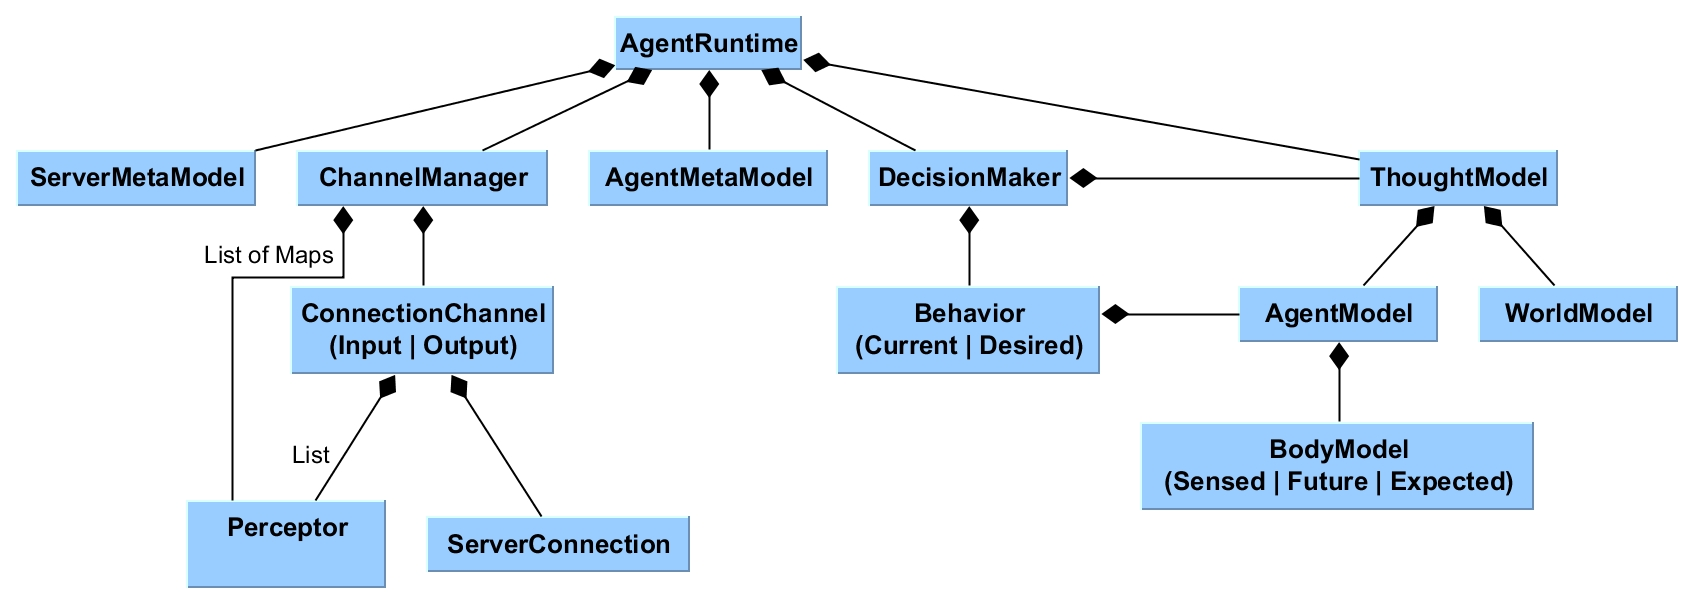
\includegraphics[width=\textwidth]{Grafiken/Magma/AgentRuntime_Structure}
	\caption{Magma Offenburg - Agent Runtime Architecture}
	\label{fig:Magma - Agent Runtime Struktur}
\end{figure}

In obiger Grafik kann man den groben Aufbau eines Magma Offenburg Agents erkennen. Die AgentRuntime ist der Java Prozess, welcher sich beim Server anmeldet und mit diesem kommuniziert. \\
\\
Für die Kommunikation ist der ChannelManager zuständig,  der die Verbindung zum Server vorhält, eingehende Daten verarbeitet (Parsen + update des Thoughtmodels) und ausgehende Daten serialisiert und an den Server weiterleitet.\\
\\
Das AgentMetaModel liefert Metainformationen über den simulierten Agent, wie verfügbare Gelenke und verfügbare Sensoren.\\
\\
Das ServerMetaModel enthält Informationen über den Server, wie aktuelle Versionsnummer, Dimensionen des Spielfelds und Namen der Landmarks.\\
\\
Hinter dem DecisionMaker verbirgt sich die komplette Logik des Agents. Der DecisionMaker entscheidet über die nächste auszuführende Behavior (Aktion). Grundlage für die Entscheidung ist das Thoughtmodel, in dem sowohl für den Spieler spezifische als auch alle Daten des Worldmodels enthalten sind.

\begin{figure}[H]
	\centering
	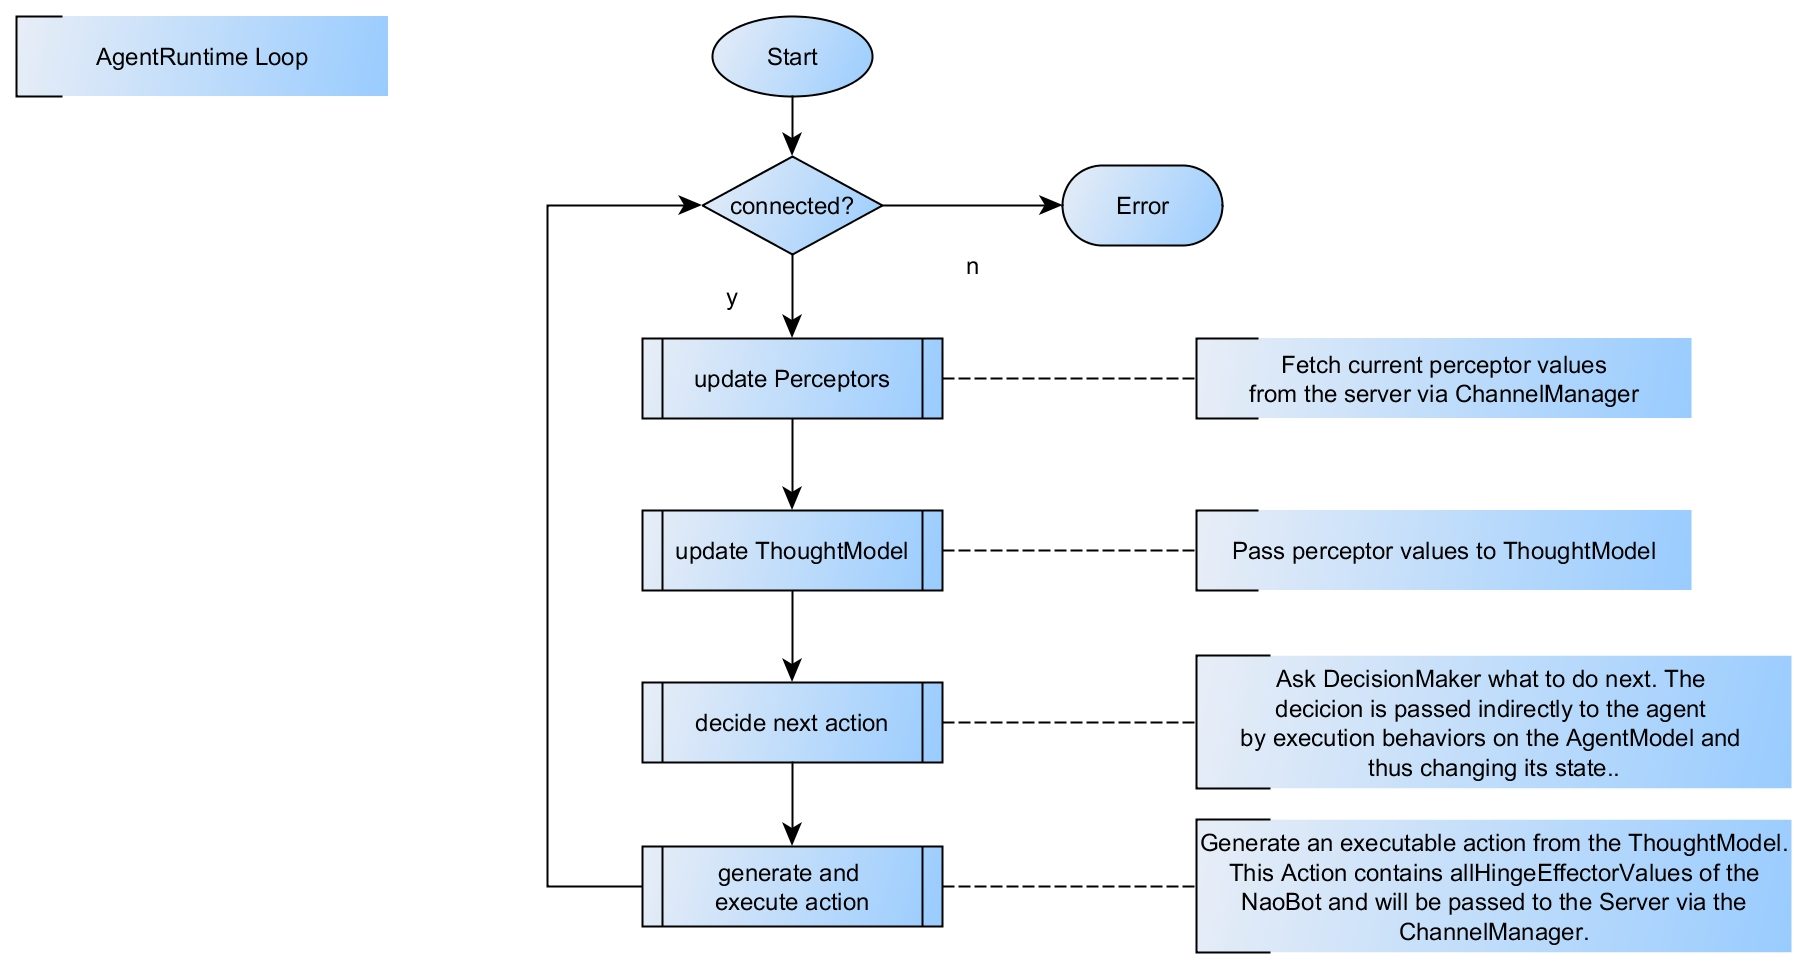
\includegraphics[width=\textwidth]{Grafiken/Magma/AgentRuntime_Loop}
	\caption{Magma Offenburg - Agent Runtime Loop}
	\label{fig:Magma - Agent Runtime Loop}
\end{figure}

Der Agent Runtime Loop beschreibt, was für jeden Zyklus im Agent passiert.\\
\\
Beim Eintreffen eines Pakets vom Server wird dessen information geparsed und die erhaltenen Werte vom ChannelManager in die Liste der Perceptors (Daten über Gelenkwinkel und Sensoren) geschrieben.
Diese werden dann in jedem Zyklus in das Thoughtmodel übernommen.\\
\\
Im Anschluss fragt der Agent seinen DecisionMaker, welche Aktion er denn ausführen soll. Dieser überprüft anhand einer Reihe von Believes, welche Behavior denn ausgehend vom aktuellen Zustand des Thoughtmodels am sinnvollsten wäre und gibt diese zurück.\\
\\
Die für den nächsten Zyklus ausführbare Behavior wird nun wieder serialisiert und vom ChannelManager an der Server gesendet.\\
\\
Mit der Antwort des Servers beginnt ein neuer Zyklus.

\begin{figure}[H]
	\centering
	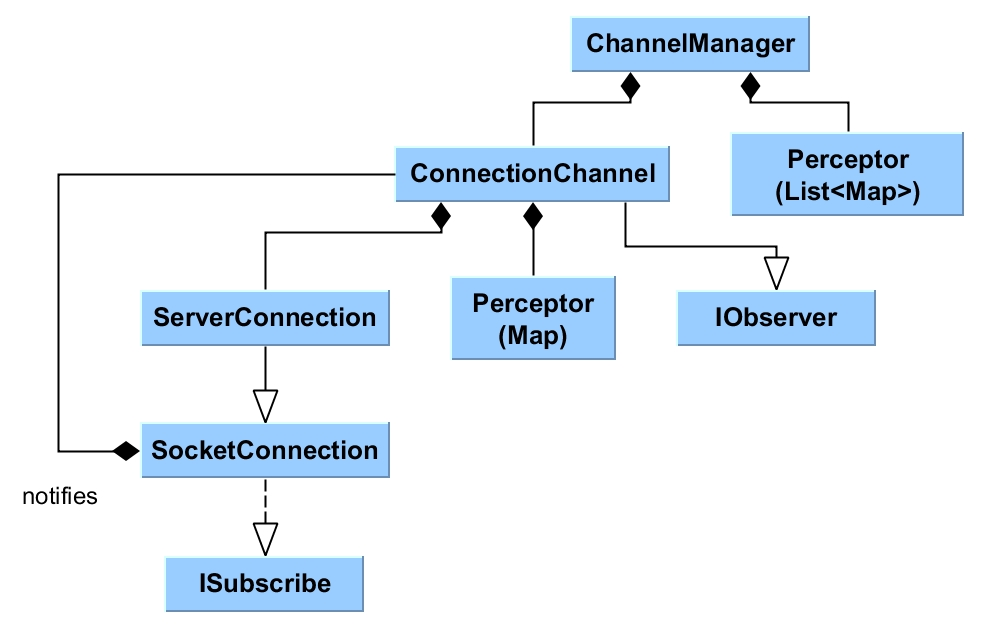
\includegraphics[width=\textwidth]{Grafiken/Magma/Observer_Structure}
	\caption{Magma Offenburg - Observer Structure}
	\label{fig:Magma - Observer Structure}
\end{figure}

Da der ChannelManager auf dem Observer Pattern basiert, möchte ich dieses noch kurz darlegen. Der ConnectionChannel meldet sich bei der SocketConnection als Observer an. Die SocketConnection hält die eigentliche Verbindung zum Server. Ist nun bei der Socket Connection ein Paket angekommen, informiert es alle seine Observer, also die ConnectionChannel, welche dann das Paket abholen, parsen und die enthaltene Information in den Perceptors abspeichern. Aus diesen werden sie dann vom Agent ausgelesen und in das Thoughtmodel übertragen. (siehe \autoref{fig:Magma - Agent Runtime Loop})

\subsubsection{Agent Startup Routine}
\textit{Verfasser: Stumpf}\\
\\
Welcher Agent mit welchen Eigenschaften gestartet werden soll ist über Kommandozeilenparameter konfigurierbar. Auf diese möchte ich im folgenden kurz eingehen:\\
\\
\texttt{--teamname="Robo1" --playerid=2 --server=192.168.56.101 --port=3100 --loglevel=severe --serverversion=68 --factory=NaoRF --decisionmaker=31 --homePosition=-15.0:0.0}\\
\\
\begin{itemize}
\item \textbf{--teamname:} Der Name des Teams. Der rcssserver3d weist Agents vom gleichen Team der gleichen Seite zu.
\item \textbf{--playerid:} Die Spielernummer. Sollte unique sein.
\item \textbf{--server:} IP-Adresse des Servers.
\item \textbf{--port:} Port auf dem der rcssserver läuft. Standard ist 3100.
\item \textbf{--loglevel:} Das Loglevel des Agents. Nur console logging, nicht grafisch.
\item \textbf{--serverversion:} Version des Servers, entscheidet welche Serverkonfigurationsdatei verwendet wird.
\item \textbf{--factory:} Die Factory entscheidet, welches Agent-Modell verwendet wird. NaoRF ist ein von unserer Grupper erstelltes Modell, welches den Nao um einiege zusätzliche Bahaviors erweitert und Fehler in den maximalen Winkeln der Gelenke behebt.
\item \textbf{--decisionmaker:} Definiert den Decisionmaker für diesen Spieler. Zuweisung erfolgt nicht besonders elegant über einen Switch-Case in der Klasse ComponentFactory.java. Fall neue DecisionMaker angelegt und verwendet werden sollen müssen diese in der ComponentFactory hinzugefügt werden. Die 31 ist der von uns entwickelte Decisionmaker, der auf dem Strategy-Role-Modell (siehe \autoref{sse:KI-Gesamtübersicht}) basiert.
\item \textbf{--homePosition:} Dieser Parameter wurde von unserer Gruppe hinzugefügt. Damit lässt sich unabhängig von der Spielernummer eine HomePosition für den zu erstellenden Agent festlegen, von welcher aus dieser agiert.
\end{itemize}

Die Kommandozeilenparameter werden über die Klasse CommandlineParser.java eingelesen. Diese wurde wohl irgendwann einmal erweitert um obige Eingabemöglichkeit. Sollte der Commandline Parser irgendeinen der obigen --<param> Parameternamen nicht kennen, so wird er auf die alte Parser Version zurückfallen, die noch keine Namen für die Parameter kennt, sondern diese in einer bestimmten Reihenfolge erwartet. Das führt zu 100\% zu einem Fehler, sollte also beachtet werden.\\
\\
Unser KI-Konzept enthält einen Strategy Decider, der seine Entscheidungen anhand von Java-VM Parametern trifft. Sollte auf dem Strategy-Role-Konzept aufgebaut werden, bzw. dieses verwendet werden (z.B. DecisionMaker ID: 31), so müssen diese für eine korrekte Funktionalität gesetzt werden.\\
\\
Beispiel eines defensiven Spielers, der ebenso Freistoß, Einwurf und Ecke spielen darf(comma-separated values):\\
\\
\texttt{-DplayableRoles=Defense,CornerKick,FreeKick,ThrowIn}\\
\\
Verfügbare Primär-Rollen:
\begin{itemize}
\item Keeper
\item Defense
\item Middle
\item Attack
\end{itemize}

Verfügbare sekundäre Rollen:
\begin{itemize}
\item CornerKick
\item FreeKick
\item GoalKick
\item ThrowIn
\item KickOff
\end{itemize}

\subsubsection{Sammlung von Agent Startup Parametern}
\textit{Verfasser: Stumpf}\\
\\
Im Folgenden möchte ich meine Sammlung an Kommandozeile- und JVM-Parametern festhalten, die zum aktuellen Zeitpunkt unserer Magma Offenburg Weiterentwicklung verwendet werden können um:
\begin{itemize}
\item Ein Team zu erstellen
	\begin{itemize}
	\item \textbf{Keeper:}\\
\texttt{JVM: -DplayableRoles=Keeper,GoalKick\\
arg: --teamname="RoboFreunde" --playerid=2 --server=127.0.0.1 --		port=3100 --loglevel=severe --serverversion=68 --factory=NaoRF --		decisionmaker=31 --homePosition=-15.0:0.0}
	\item \textbf{Defense:}\\
\texttt{JVM: -DplayableRoles=Defense,CornerKick,FreeKick,ThrowIn}\\
\textbf{-Left:}\\
\texttt{arg: --teamname="RoboFreunde" --playerid=2 --server=127.0.0.1 --port=3100 --loglevel=severe --serverversion=68 --factory=NaoRF --decisionmaker=31 --homePosition=-10.0:5.0}\\
\textbf{-Mid:}\\
\texttt{arg: --teamname="RoboFreunde" --playerid=6 --server=127.0.0.1 --port=3100 --loglevel=severe --serverversion=68 --factory=NaoRF --decisionmaker=31 --homePosition=-10.0:0.0}\\
\textbf{Right:}\\
\texttt{arg: --teamname="RoboFreunde" --playerid=3 --server=127.0.0.1 --port=3100 --loglevel=severe --serverversion=68 --factory=NaoRF --decisionmaker=31 --homePosition=-10.0:-5.0}
	\item \textbf{MidField:} NOTE: Es wird abgeraten den Mittelfeldspieler zu verwenden, da dieser zum aktuellen Zeitpunkt unzureichend funktioniert!\\
\texttt{JVM:-DplayableRoles=Middle,CornerKick,FreeKick,ThrowIn,KickOff}\\
\textbf{-Left:}\\
\texttt{arg: --teamname="RoboFreunde" --playerid=8 --server=127.0.0.1 --port=3100 --loglevel=severe --serverversion=68 --factory=NaoRF --decisionmaker=31 --homePosition=-7.0:-4.0}\\
\textbf{-Mid:}\\
\texttt{arg: --teamname="RoboFreunde" --playerid=9 --server=127.0.0.1 --port=3100 --loglevel=severe --serverversion=68 --factory=NaoRF --decisionmaker=31 --homePosition=-7.0:0.0}\\
\textbf{Right:}\\
\texttt{arg: --teamname="RoboFreunde" --playerid=10 --server=127.0.0.1 --port=3100 --loglevel=severe --serverversion=68 --factory=NaoRF --decisionmaker=31 --homePosition=-7.0:4.0}
	\item \textbf{Attack:}\\
\texttt{JVM: -DplayableRoles=Attack,CornerKick,FreeKick,ThrowIn,KickOff}\\
\textbf{-Left:}\\
\texttt{arg: --teamname="RoboFreunde" --playerid=4 --server=127.0.0.1 --port=3100 --loglevel=severe --serverversion=68 --factory=NaoRF --decisionmaker=31 --homePosition=-4.0:2.5}\\
\textbf{-Mid:}\\
\texttt{arg: --teamname="RoboFreunde" --playerid=7 --server=127.0.0.1 --port=3100 --loglevel=severe --serverversion=68 --factory=NaoRF --decisionmaker=31 --homePosition=-2.0:0.0}\\
\textbf{-Right:}\\
\texttt{arg: --teamname="RoboFreunde" --playerid=5 --server=127.0.0.1 --port=3100 --loglevel=severe --serverversion=68 --factory=NaoRF --decisionmaker=31 --homePosition=-3.0:-2.5}
	\end{itemize}
\item Challenges zu starten
	\begin{itemize}
	\item \textbf{Kicks to Goal Challenge:}\\
\texttt{arg: --teamname="RoboFreunde" --server=127.0.0.1 --playerid=2 --port=3100 --loglevel=severe --serverversion=68 --factory=NaoRF --decisionmaker=12 --homePosition=-2.0:0.0}
	\item \textbf{Time to Goal Challenge:}\\
\texttt{arg: --teamname="RoboFreunde" --server=127.0.0.1 --playerid=2 --port=3100 --loglevel=severe --serverversion=68 --factory=NaoRF --decisionmaker=14 --homePosition=-2.0:0.0}
	\end{itemize}
\item Metrik-Agents zu starten
	\begin{itemize}
	\item \textbf{Kick Evaluation:}\\
\texttt{arg: --teamname="RoboFreunde" --server=127.0.0.1 --playerid=2 --port=3100 --loglevel=severe --serverversion=68 --factory=NaoRF --decisionmaker=26 --homePosition=-2.0:0.0}
	\item \textbf{Run Evaluation:}\\
\texttt{arg: --teamname="RoboFreunde" --playerid=2 --server=127.0.0.1  --port=3100 --loglevel=severe --serverversion=68 --factory=NaoRF --decisionmaker=13}
	\item \textbf{Dribble Evaluation:}\\
\texttt{arg: --teamname="RoboFreunde" --playerid=2 --server=127.0.0.1  --port=3100 --loglevel=severe --serverversion=68 --factory=NaoRF --decisionmaker=23}
	\item \textbf{Manual Keyboard Bot:} NOTE: Dieser Bot lässt sich mit einem Gamepad steuern. Unterstützt wird der XBox-Controller. Gedacht ist es, damit einen Agent in gewünschte Spielposition zu bringen und seine Reaktion zu testen.\\
\texttt{arg: --teamname="RoboFreunde" --playerid=2 --server=127.0.0.1  --port=3100 --loglevel=severe --serverversion=68 --factory=NaoRF --decisionmaker=100}
	\end{itemize}
\end{itemize}

\subsubsection{Verschiedene NAO-Models}
\textbf{-> TODO: Felix}

\subsubsection{DecisionMaker, Believes, Behaviors}
\textit{Verfasser: Stumpf}\\
\\
DecisionMaker, Believes un Behaviors sind in Magma Offenburg ein eng verwobenes Konstrukt. Der DecisionMaker hat die Aufgabe, die Entscheidung über die nächste auszuführende Aktion zu treffen. Das zu implementierende Interface ist IDecisionMaker und definiert zwei relevante Methoden:
\begin{itemize}
\item \texttt{boolean decide();} Wird aufgerufen, wenn der DecisionMaker anhand des aktuellen Thoughtmodels eine Entscheidung über die nächste Aktion treffen soll. Überschreibt currentBehavior.
\item \texttt{IBehavior getCurrentBehavior();} Gibt die aktuell auszuführende Aktion currentBehavior zurück.
\end{itemize}

Die konkrete Implementierung des DecisionMakers kennt die Instanz des Thoughtmodels und hat somit immer Zugriff auf alle aktuellen Informationen. Die konkrete Entscheidung der nächsten Aktion ist ausgelagert in die Believes, wie man an folgendem Codeausschnitt der Implementierung von \texttt{decide()} sehen kann.
\begin{lstlisting}[caption=Ausschnitt aus decide(), captionpos=b, label=lst:DecidionMaker - decide()]
.
.
.
void decide() {
	.
	.
	.
	IBehavior toExecute = null;

	// temperature cool down
	toExecute = temperatureCoolDown();
	if (toExecute != null) {
		return toExecute;
	}
	// what to do when the game is finished
	toExecute = gameEndedAction();
	if (toExecute != null) {
		return toExecute;
	}
	// beam to this players starting position if it is allowed
	toExecute = beamHome();
	if (toExecute != null) {
		return toExecute;
	}
	.
	.
	.
	currentBehavior = toExecute;
}
.
.
.
protected IBehavior temperatureCoolDown()
{
	IBelief tooHot = believes.get(IBeliefConstants.TEMPERATURE_HOT);
	if (tooHot.getTruthValue() > 0.7) {
		return behaviors.get(IBehaviorConstants.SHUT_OFF);
	}
	if (tooHot.getTruthValue() > 0.4) {
		return behaviors.get(IBehaviorConstants.MOVE_ZERO);
	}
	return null;
}
.
.
.
\end{lstlisting}

Wie man in obigem Codeausschnitt sehen kann, werden der Reihe nach, nach Prioritäten geordnet, verschiedene Believes abgefragt. Sollte eine der Believes zutreffen, oder über einem Schwellwert sein (siehe Methode \texttt{temperatureCoolDown()}), so wird die damit verknüpfte Behavior zurückgegeben. Eine Behavior ist Zusammengesetzt aus Movements, von denen jede eine Reihe von gewünschten Winkelpositionen verschiedener Gelenke enthält, sowie Informationen in wie vielen Cycles und mit welcher Geschwindigkeit diese erreicht werden. Eine Behavior definiert somit einen Bewegungsablauf.
Beispiele für Behaviors sind:
\begin{itemize}
\item Aufstehen
\item Laufen
\item Kicken
\item Sich ausschalten
\item Nichts tun
\item Ball fokussieren
\item usw.
\end{itemize}

Meist prüfen die Behaviors selbst noch einmal, ob das mit ihnen verknüpfte Belief auch zutrifft. Zum Beispiel wird der Kick nur ausgeführt, wenn der Ball auch Kickable ist (Siehe Belief BallKickable). Falls nicht wird entweder die NullBehavior zurückgegeben, also nicht getan oder ein Fehler geworfen.

\subsubsection{Thought- und Worldmodel}
\textit{Verfasser: Stumpf}\\
\\
Das Thoughtmodel steht für die Datenhaltung des Agents. Es definieren den Zustand, in dem sich der Agent und das aktuelle Spiel gerade befinden. Nicht alle Daten sind im Thoughtmodel selbst enthalten, es fungiert jedoch als Container für Worldmodel, Flagmodel und Agentmodel. Das Worldmodel ist hiervon das wichtigste, da es die meisten Informationen enthält. Die Kommunikation über das Say-Interface des Servers wird praktischerweise ausgenutzt, um das Worldmodel aller eigenen Agents möglichst konsistent zu halten. Die Spieler tauschen darüber Informationen wie die eigene Position aus, die dann mit dem Worldmodel der anderen Spieler abgeglichen wird.
Positionen im Worldmodel sind immer aus Sicht des eigenen Teams angegeben. Der Ursprung des Koordinatensystems ist der Mittelpunkt des Spielfeldes. Die eigene Hälfte liegt dann im negativen Bereich der X-Achse, die gegnerische im positiven. Vom eigenen Tor aus gesehen links entspricht positiven Werten auf der Y-Achse, rechts negativen.\\
\\
Im Folgenden einige Thoughtmodel spezifische Informationen, diese stehen immer in Bezug zum eigenen Agent:
\begin{itemize}
\item \texttt{getObstacles()} Hindernisse, die ich (eigener Agent) umgehen muss.
\item \texttt{getPlayersAtMe()} Alle Spieler, geordnet nach Abstand zu mir.
\item \texttt{getOpponentsAtMe()} Alle Gegner, geordnet nach Abstand zu mir.
\item \texttt{...}
\end{itemize}

Das Worldmodel enthält die meisten für das Spiel relevanten Informationen:
\begin{itemize}
\item \texttt{Ball getBall()} Das Ball Objekt enthält Informationen über den Ball (u.a. seine Position).
\item \texttt{Vector3D getOwn/OpponentGoalPosition()} Position des eigenen/gegnerischen Tors. 
\item \texttt{GameState getGameState()} Spielstatus als Enum.
\item \texttt{PlaySide getPlaySide()} Spielfeldseite als Enum.
\item \texttt{float getGameTime()} Spielzeit.
\item \texttt{int getGoalsWe/TheyScored()} Anzahl der eigenen/gegnerischen Tore.
\item \texttt{...}
\end{itemize}

\subsubsection{Server Kommunikation}
\textbf{-> TODO: Felix}

\section{KI-Konzept}
\textit{Verfasser: Wurth}\\

Für die KI wurde ein Konzept entwickelt, dass sich einfach in die bereits existierende Architektur des verwendeten Frameworks integrieren ließ. Ziel war es, eine möglichst flexible und gleichzeitig einfache Architektur zu entwerfen. Das Ergebnis ist eine Schichten-Architektur, deren Teilkomponenten einfach verändert oder ausgetauscht werden können. Nebeneffekte auf andere Module sind durch die Architektur weitgehend ausgeschlossen. So war es beispielsweise Problemlos möglich, verschiedene Herangehensweisen für die Implementierung von Rollen in das Gesamtsystem zu integrieren. Verschiedene Teammitglieder konnten also ihre selbst entwickelten Rollen schnell und einfach in das Gesamtsystem integrieren, ohne andere Komponenten anpassen zu müssen.

\subsection{Anforderungen}
\textit{Verfasser: Wurth}\\

Das gewählte Framework und die Tatsache, dass eine Steuerung für eigenständige Roboter entwickelt werden musste, stellt einige Anforderungen an die zu entwickelnde künstliche Intelligenz.\\
\\
Jeder Roboter ist als unabhängiges Individuum zu verstehen. Das hat die direkte Folge, dass Entscheidungen nicht von einer übergeordneten Instanz getroffen werden können; Jeder Roboter muss aufgrund der ihm zur Verfügung stehenden Informationen seine eigenen Entscheidungen treffen. Das Fehlen einer zentralen Komponente erschwert es erheblich, ein aufeinander abgestimmtes Team-Spiel zu entwickeln. Dennoch gibt es für dieses Problem gute Ansätze. Die Anforderung, die sich zusammenfassend daraus ableiten lässt, ist die Notwendigkeit einer dezentralen Lösung für die KI.\\
\\
Eine weitere Anforderung ergibt sich aus der Wahl des Frameworks. Das Framework arbeitet weitgehend mit Polling, also einem kontinuierlichen Abfragen der nächsten Aktion. Es ist daher naheliegend, auch für die hier zu entwickelnde KI einen Ansatz mit Polling zu zu verfolgen.\\
\\
Neben den mehr oder weniger durch die äußeren Umstände vorgegebenen Anforderungen haben wir noch weitere zwei Anforderungen definiert. Roboter sollen ihre Rolle dynamisch wechseln, außerdem soll es zusätzlich die Möglichkeit geben, die aktuell verfolgte Spiel-Strategie nach Bedarf zu ändern.

\subsection{Komponenten}
\textit{Verfasser: Wurth}\\

Das KI-Grundkonzept besteht aus insgesamt 4 Schichten. Jede Schicht kennt ausschließlich die darunterliegende Schicht. Die unterste Ebene definiert Grundlegende Bewegungen eines Roboters. Direkt darüber befinden sich Rollen. Rollen sind zum Beispiel \glqq Stürmer\grqq oder \glqq Torwart\grqq, aber auch Spezialrollen wie \glqq Anstoß\grqq oder \glqq Freistoß\grqq. Über den Rollen befindet sich die Strategie-Ebene. Auf höchster Ebene befindet sich der Strategie-Entscheider.

\subsubsection{Elementare Bewegungen}
\textit{Verfasser: Wurth}\\

Elementare Bewegungen sind die Grundlage für alle höheren Schichten. Sie sind die unmittelbare Voraussetzung die darüber liegenden Rollen, weil sie von diesen direkt benutzt werden. Elementare Bewegungen sind zum Beispiel: \glqq Laufen\grqq, \glqq Aufstehen\grqq, \glqq Schießen\grqq, oder \glqq Dribbeln\grqq. Abgesehen vom \glqq Dribbeln\grqq waren alle Bewegungen bereits mehr oder weniger funktionsfähig im Framework vorhanden. Dennoch musste an einigen Stellen optimiert und angepasst werden, siehe Kapitel \ref{se:Elementare Bewegungen}.

\subsubsection{Rollen}\label{Rollen Konzept}
\textit{Verfasser: Wurth}\\

Rollen definieren das Grundlegende Verhalten eines Roboters. Ein Verteidiger verfolgt eine andere Spielweise als ein Torwart. Alle unsere Rollen sind Statemachines. Eine wichtige Frage ist, wo und wie die KI für Standard-Situationen wie zum Beispiel den \glqq Anstoß\grqq in der Architektur verankert werden soll. Eine naheliegende Lösung ist die Definition von Spezialrollen, die genau diese Standard-Situationen behandeln. Die Alternative wäre eine Erweiterung aller Standard-Rollen um die Algorithmik der Standard-Situationen. Einen wirklichen Mehrwert hat man dadurch allerdings nicht, denn der Algorithmus um einen Anstoß zu machen benötigt keine Routinen eines Stürmers. Umgekehrt gilt das Selbe. Die Entscheidung fiel also auf die Definition von Spezialrollen, die genau diese Standard-Situationen umsetzen. Ein Spieler, der normalerweise zum Beispiel Stürmer ist, wechselt bei Bedarf einfach seine Rolle in \glqq Anstoß\grqq{} und im Anschluss wieder zurück.

\begin{figure}[H]
	\centering
	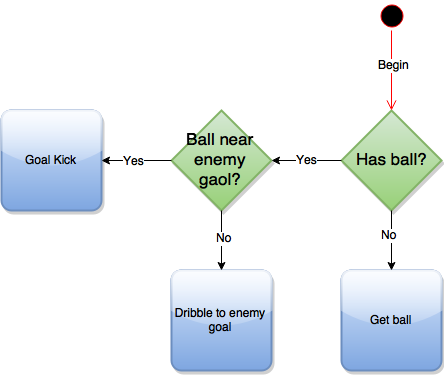
\includegraphics[width=0.7\textwidth]{Grafiken/KI/simple_Player}
	\caption{Beispiel Rolle: Einfacher Torwart}
	\label{Simple keeper}
\end{figure}

Abbildung \ref{Simple keeper} zeigt Beispielhaft den Entscheidungsbaum eines einfachen Torwarts.

\subsubsection{Strategien}
\textit{Verfasser: Wurth}\\

Rollen sollen nicht selbst entscheiden, ob und in welche andere Rolle gewechselt wird. Das widerspräche der Schichtenarchitektur. Deshalb wurde die darüber liegende Strategieschicht eingeführt. Die Aufgabe dieser Schicht ist es, Rollen dynamisch zuzuordnen. Daher ist die Bezeichnung \glqq Strategie\grqq auch treffend; Eine Strategie steuert unter Anderem die Gesamtaufstellung des Teams. Damit lässt sich die allgemeine Spielweise des gesamten Teams steuern, mehr Verteidiger bedeutet eine defensive, mehr Angreifer eine aggressive Strategie. Eine Strategie benötigt einen Pool an Rollen, die sie \glqq verteilen\grqq darf. Dieser Pool definiert die grundlegende Spielweise eines Teams. Aufgabe jeder Strategie ist es dann, Rollen dynamisch nach Bedarf zu verteilen. Darunter fällt auch die Vergabe der Spezialrollen.

\subsubsection{Strategie-Entscheider}
\textit{Verfasser: Wurth}\\

In der Strategieebene können verschiedene Strategien für verschiedene Gesamtaufstellungen des Teams definiert werden. Im Laufe eines Spiels kann es sinnvoll sein, die Aufstellung an die Gegebenheiten und Anforderungen an das Spiel anzupassen. Dafür Wurde auf höchster Ebene ein Entscheidungsmechanismus etabliert. Die Aufgabe dieser Schicht ist es, je nach Bedarf eine passende Strategie auszuwählen. Dafür gibt es verschiedene Ansätze, zum Beispiel könnte eine passende Strategie je nach aktuellem Spielstand ausgesucht werden. Beispiel: 
\begin{itemize}
\item Mannschaft liegt vorne: Defensive Strategie
\item Unentschieden: Aggresive Strategie
\item Mannschaft liegt hinten: Aggressive Strategie
\item Mannschaft liegt hinten und Zeit läuft bald aus: Risiko Strategie
\end{itemize}

\begin{figure}[H]
	\centering
	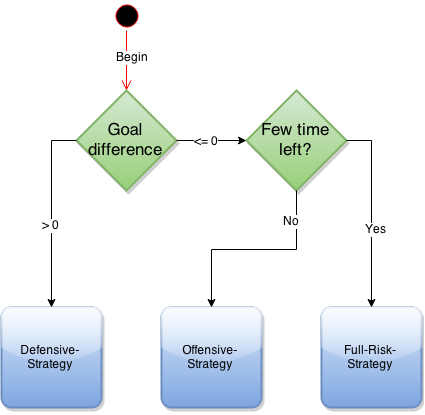
\includegraphics[width=0.7\textwidth]{Grafiken/KI/SimpleStrategyDecider}
	\caption{Einfacher Strategie Entscheider}
	\label{Einfacher Strategie Entscheider}
\end{figure}

Abbildung \ref{Einfacher Strategie Entscheider} zeigt den Enscheidungsbaum eines sehr einfachen Entscheidungsmeachanismus für Strategien.

\subsection{Gesamtübersicht}\label{sse:KI-Gesamtübersicht}
\textit{Verfasser: Wurth}\\

\begin{figure}[H]
	\centering
	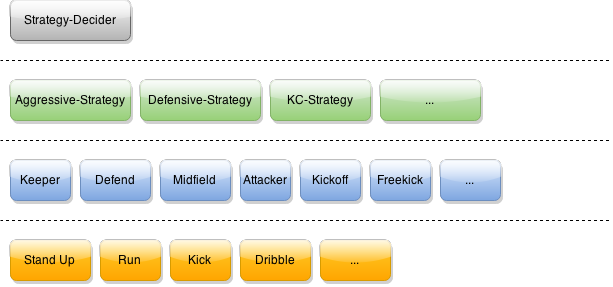
\includegraphics[width=\ScaleIfNeeded]{Grafiken/KI/Ki-Concept}
	\caption{Gesamtkonzept KI}
	\label{Gesamtkonzept KI}
\end{figure}

Abbildung \ref{Gesamtkonzept KI} zeigt das Gesamtkonzept mit allen 4 Ebenen. Ganz unten befinden sich die elementaren Bewegungen. Rollen werden auf der Schicht darüber definiert. Sie greifen als einzige Schicht auf elementare Bewegungen direkt zu. Über den Rollen befindet sich die Strategie-Ebene. Jede Strategie hält einen Pool an Rollen vor und Steuert damit die konkrete Aufstellung auf dem Spielfeld. Auf höchster Ebene befindet sich der Entscheidungsmechanismus, der Situationsabhängig eine passende Strategie aktiviert. 


\section{Elementare Bewegungen}\label{se:Elementare Bewegungen}
\textit{Verfasser: Stumpf}\\
\\
Im Laufe der Entwicklung hat sich herausgestellt, dass die in Magma Offenburg verfügbare Behaviors unzureichend waren für unsere Anforderungen.\\
\\
Es mangelte entweder an Funktionalität, oder an der Performance der Bewegungsabläufe. So war zum Beispiel weder Dribbeln, noch der Kick zu einer gegebenen Position implementiert und die Behaviors für Laufen und Kicken funktionierten denkbar schlecht.\\
\\
Es wurde demnach ein Teil des Teams mit der Implementierung und Optimierung benötigter Bewegungsabläufe beauftragt.

\subsection{Anforderungen}
\textit{Verfasser: Stumpf}\\
\\
Die Anforderungen an die neuen Behaviors kamen zum Teil aus dem KI-Team. So sind Dribbeln und ein Kick zu gegebener Position (KickToPosition) von den KI's vorausgesetzte Behaviors.\\
\\
Es fielen jedoch auch offensichtliche Mängel an einigen Behaviors auf, die es zu beheben galt. So war das Laufen von Magma Offenburg anfangs genau so wenig zu gebrauchen wie die implementierten Kicks.\\
\\
Mittels entwickelter Metriken und diese umsetzenden Metrik-Agents wurden die neuen und optimierten Behaviors mit den alten verglichen und getestet, um die Verbesserungen sichtbar zu machen. Sehr wichtig dafür war die Möglichkeit des grafischen Debugging mit RoboViz. (siehe \autoref{se:Grafisches Debugging})

\subsection{Laufen}\label{sse:Elem Bew:Laufen}
\textbf{-> TODO: Felix}
\subsection{Dribbeln}\label{sse:Elem Bew:Dribbeln}
\textbf{-> TODO: Felix}
\subsection{Schie{\ss}en}\label{sse:Elem Bew:Schiessen}
\textbf{-> TODO: Stumpfi}
\subsubsection{Behaviors}
\textbf{-> TODO: Stumpfi}
\subsubsection{Evaluierung, Metrik Bots}
\textbf{-> TODO: Stumpfi}

\section{Rollen}
\textit{Verfasser: Wurth}\\

Rollen legen fest, welches übergeordnete Ziel ein Roboter zu einem bestimmten Zeitpunkt verfolgt aber vor Allem, wie dieses Ziel erreicht werden soll. Ziele wie Aufstehen nach einem Sturz, oder die eigene Position vor dem Ball korrigieren, sind untergeordnete Ziele die vor allem in den elementaren Bewegungen verfolgt werden. Ein Stürmer, dessen finales Ziel es ist, ein Tor zu schießen, muss natürlich einige Schritte Vorarbeit zum Erreichen dieses Ziels leisten. Zum Beispiel muss er zuerst den Ball erobern. Die Algorithmik, die zum Erreichen eines solchen Ziels erforderlich ist, findet ihren Platz in den Rollen. Wie in Kapitel \ref{Rollen Konzept} bereits erwähnt, werden Rollen in zwei Kategorien unterteilt, nämlich Standard-Rollen und Spezial-Rollen.
\\

Unter Standardrollen fallen alle normalen Spielertypen wie Stürmer, Verteidiger oder Torwart. In diesem Projekt wurden insgesamt 4 Standardrollen implementiert, deren genauere Beschreibung in diesem Kapitel Platz findet. Die Implementierung der Standardrollen wurde von verschiedenen Team-Mitgliedern durchgeführt. Stürmer und Torwart wurden von einer Person, Verteidiger und Mittelfeldspieler auch von jeweils einer Person entwickelt. Die Herangehensweisen unterscheiden sich deshalb zwischen den Rollen stark.
\\

Spezialrollen wiederum kümmern sich um spezielle Situationen wie zum Beispiel den Anstoß oder den Kick-In.


\subsection{Standardrollen: Torwart und Stürmer}
\textit{Verfasser: Wurth}\\

Die Rolle Torwart und die Rolle Stürmer wurden von einer Person entwickelt. Sie teilen sich deshalb ein gemeinsames Grundkonzept.

\subsubsection{Konzept}
\textit{Verfasser: Wurth}\\

Wie alle anderen Rollen auch, sind die Rollen für Torwart und Stürmer State-Machines. Jede State-Machine beinhaltet mehrere States. Jeder State hat eine ganz bestimmte Aufgabe, zum Beispiel: Zu einer bestimmten Position laufen. Im Kern befindet sich innerhalb eines States nur die Parametrisierung einer konkreten elementaren Bewegung. Diese Bewegung kann dann mittels Poll von außen abgefragt werden.
\\

Der erste Ansatz zur Modellierung der State-Machine war klassisch; Jeder State hatte eine bestimmte Menge an Folgestates und konnte demzufolge ausschließlich in diese States übergehen. Nach und nach offenbarte sich aber die Problematik dieser Designentscheidung. Bei laufenden Tests viel auf, dass bestimmte Transitionen von einem in einen anderen State nicht bedacht wurden. Folglich musste die State-Machine überarbeitet werden. Das führte recht schnell zu einer anderen Herangehensweise; Jeder State hat jeden anderen State der State-Machine als potenziellen Nachfolger. Ein enormer Flexibilitätszuwachs zur ersten Variante. Jetzt konnte der Entscheidungsmechanismus zur Findung des nächsten States  zentral etabliert werden. 
\\

Dazu wurde für beide Rollen jeweils eine Basisklasse angelegt. Diese Klasse kümmert sich um das Vorhalten aller States der StateMachine. Außerdem findet in ihr die Methode Platz, die einen Folgestate auswählt. Diese Methode ist das Herzstück der Rolle, sie definiert was wann gemacht werden soll.
\\

\begin{lstlisting}[caption=Beispiel Basisklasse Stürmer, captionpos=b, label=Beispiel Basisklasse Stürmer]
public abstract class BaseAttackerCenter extends BaseState {
    private DribbleState dribbleState;
    private GoalKickState goalKickState;
    private GoToBallState goToBallState;
    private GoToPositionState goToPositionState;
    private PassState passState;

    public void bootstrap(DribbleState dribbleState, 
    					  GoalKickState goalKickState, 
    					  GoToBallState goToBallState, 
                          GoToPositionState goToPositionState, 
                          PassState passState) 
    {
        this.dribbleState = dribbleState;
        this.goalKickState = goalKickState;
        this.goToBallState = goToBallState;
        this.goToPositionState = goToPositionState;
        this.passState = passState;
    }

    public BaseState decideNextState() {
        ...
    }
}
\end{lstlisting}

Listing \ref{Beispiel Basisklasse Stürmer} zeigt den Aufbau einer Basisklasse für States am Beispiel des Stürmers. Sie bekommt in der Methode \lstinline$bootstrap()$ von außen alle States und hält sie dann vor. Außerdem befindet sich ab Zeile 21 die Methode \lstinline$decideNextState()$.

Jeder Konkrete State leitet von diesem Basis-State ab und erbt somit alle States der Statemachine sowie die Methode \lstinline$decideNextState()$.
\\

\begin{lstlisting}[caption=Beispiel eines konkreten States: GoToBallState, captionpos=b, label=Beispiel eines konkreten States: GoToBallState]
public class GoToBallState extends BaseAttackerCenter {
    IBehavior moveToBall;

    @Override
    public void init(Player player) {
        super.init(player);
        this.moveToBall = null;
    }

    @Override
    public BotState update() {
        BaseState nextState = decideNextState();

        if (nextState == this) {
            RunToPosition moveToBall = (RunToPosition) getPlayer().getBehavior(IBehaviorConstants.RUN_TO_POSITION);
            moveToBall.setPosition(calcProperRunToBallPose(), 0, 0, 75, false);
            this.moveToBall = moveToBall;
            return null;
        }
        return nextState;
    }

    @Override
    public IBehavior getBehavior() {
        return this.moveToBall;
    }
}
\end{lstlisting}

Listing \ref{Beispiel eines konkreten States: GoToBallState} zeigt Beispielhaft den State, der für das Laufen zum Ball verantwortlich ist. Er hält eine sogenannte \lstinline$IBehavior$ vor, die am Ende für das Ausführen der Bewegung benötigt wird. Innerhalb des States findet also nicht die Ausführung der Bewegung statt, sondern nur deren Parametrisierung. In der \lstinline$update()$-Methode passiert in Zeile 12 zuerst die Abfrage des für die aktuelle Situation besten States. Dazu wird die geerbte Methode \lstinline$decideNextState()$ aufgerufen. Nur wenn der zurückgegebene State er selbst ist, soll er seinen Code ausführen und die \lstinline$IBehavior$ bearbeiten (Zeilen 14 - 18). Wurde ein anderer State zurückgegeben, wird kein eigener Code ausgeführt und der neue State zurückgegeben (Zeile 20). Damit die \lstinline$IBehavior$ von außen abgerufen werden kann, wurde hierfür ein Getter erzeugt (Zeilen 23 - 26).

\subsubsection{Standardrolle: Torwart}
\textit{Verfasser: Wurth}\\

\begin{figure}[H]
	\centering
	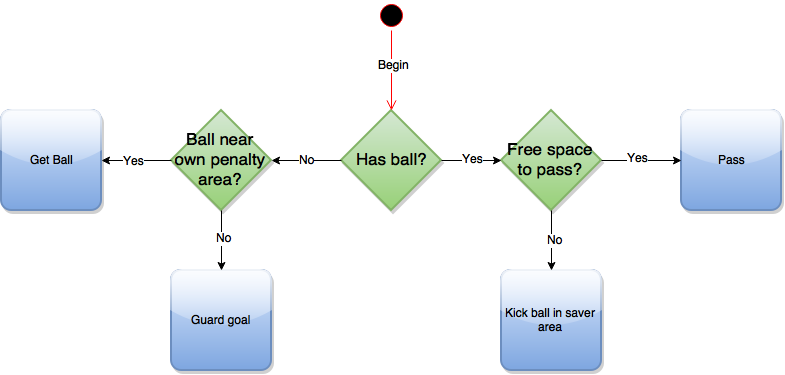
\includegraphics[width=\ScaleIfNeeded]{Grafiken/KI/Keeper}
	\caption{Torwart Entscheidungsbaum}
	\label{Torwart Entscheidungsbaum}
\end{figure}

Abbildung \ref{Torwart Entscheidungsbaum} zeigt den Entscheidungsbaum des Torwarts. Die Entscheidungsbäume von Torwart und Stürmer finden ihre direkte Umsetzung in der \lstinline$decideNextState()$ des Basis-States. Es war also sehr sinnvoll vor der Implementierung derartige Entscheidungsbäume zu entwerfen.
\\

Die Statemachine des Torwarts besteht aus insgesamt 4 States. Die erste Überprüfung ist, ob der Spieler den Ball besitzt. Besitzt er den Ball, will er ihn schnell wieder loswerden, schließlich ist er ein Torwart. Dazu Sucht er im eigenen Team passende Passpartner. Ein passender Passpartner steht in einer passenden Entfernung und wird nicht von einem gegnerischen Spieler geblockt. Ist ein passender Spieler gefunden wird der Pass ausgeführt. Findet sich kein Spieler, soll der Ball in Richtung der Mittellinie geschossen werden, also möglichst weit weg von eigenen Tor.
\\

Besitzt der Torwart den Ball nicht, kommt es darauf an wie weit der Ball weg ist. Ist der Ball ein gutes Stück entfernt, soll in den State \lstinline$GuardGoalState$ gewechselt werden. Was dieser State genau macht wird später beschrieben. Kommt der Ball dem eigenen Tor zu Nahe, soll der Torwart reagieren und auf den Ball zulaufen um ihn zu erobern.
\\

\textbf{Der \lstinline$GuardGoalState$}
\\

Hat der Ball eine relativ große Entfernung zum Tor, soll sich der Torwart natürlich nicht vom eigenen Tor wegbewegen. Vielmehr sollte er eine geeignete Position vor dem Tor einnehmen. Ziel ist es, eine möglichst große Fläche des Tors zu \glqq verdecken\grqq, um Distanzschüsse zu verhindern oder zumindest zu erschweren. Dafür ist der \lstinline$GuardGoalState$ zuständig.
\\

\begin{figure}[H]
	\centering
	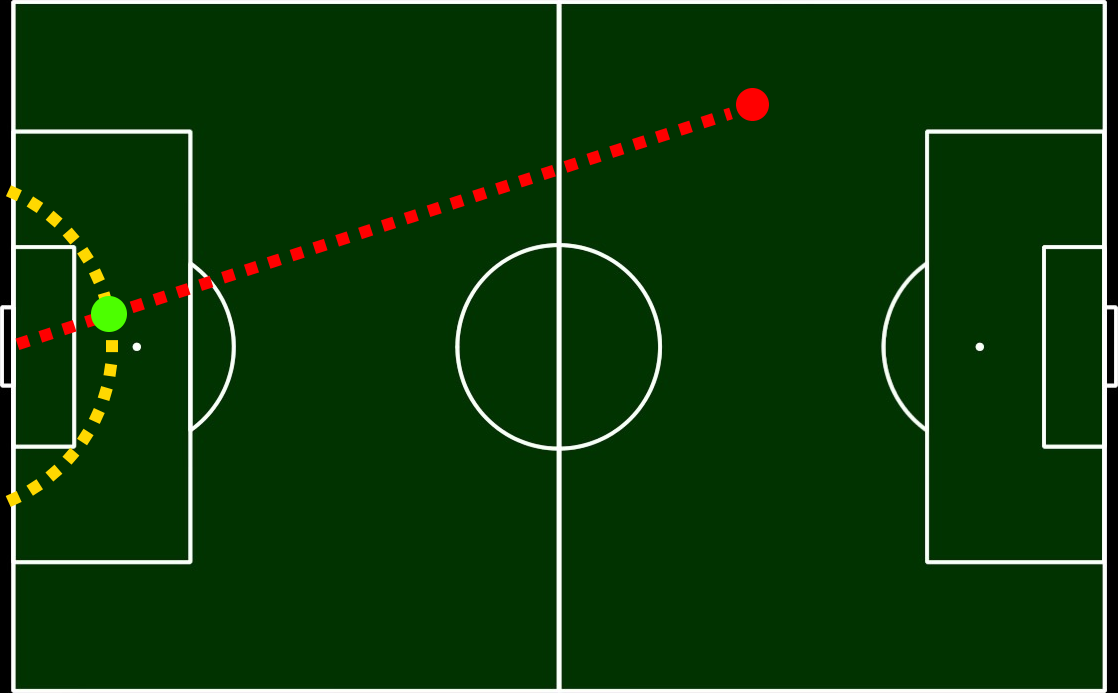
\includegraphics[width=\ScaleIfNeeded]{Grafiken/KI/guard_goal}
	\caption{Veranschaulichung des \lstinline$GuardGoalState$s}
	\label{Veranschaulichung des GuardGoalState}
\end{figure}

Abbildung \ref{Veranschaulichung des GuardGoalState} veranschaulicht die Berechnung der optimalen Position vor dem Tor anhand einer Grafik. Der gelbe Halbkreis definiert alle möglichen Positionen vor dem Tor, die der Torwart im \lstinline$GuardGoalState$ einnehmen kann. Die genaue Position hängt von der aktuellen Position des Balls ab. Dazu wird eine Gerade vom Ball in das Eigene Tor gelegt, der Schnittpunkt mit dem gelben Halbkreis entspricht der optimalen Position.
\\

\begin{lstlisting}[caption=Umsetzung des \lstinline$GuardGoalState$s, captionpos=b, label=Umsetzung des GuardGoalState]
public Vector3D getGoodGoalieDefendPosition() {  
	Vector3D ballPosition = thoughtModel.getWorldModel().getBall().getPosition();  
	Vector3D goalPosition = thoughtModel.getWorldModel().getOwnGoalPosition();    
	Vector3D direction = ballPosition.subtract(goalPosition);  
	direction = direction.normalize().scalarMultiply(2.0f);  
	return goalPosition.add(direction);  
}  

\end{lstlisting}

Listing \ref{Umsetzung des GuardGoalState} zeigt die Berechnung der korrekten Position im Code. Notwendig sind jeweils die Position des Ball und des eigenen Tors (Zeilen 2 und 3). Dann wird ein Richtungsvektor berechnet, der vom Tor Richtung Ball zeigt (Zeile 4). Dieser wird zuerst normiert und dann auf die Länge 2 skaliert. Der Abstand 2 vom Tor hat sich als guter Wert herausgestellt (Zeile 5). Die gesuchte Position errechnet sich durch die Addition des Richtungsvektors auf die Torkoordinate (Zeile 6).
\\

\textbf{Energiesparmaßnahme}
\\
Der Torwart wird die meiste Zeit innerhalb des \lstinline$GuardGoalState$ bleiben. Bei jedem Poll wird eine neue Position anhand der Ball und Torposition berechnet, zu der er dann hinläuft. Bei Ball und Torkoordinate handelt es sich aber um circa Angaben, schließlich wird das Worldmodel anhand der Sensoren des Roboters kontinuierlich korrigiert. Dabei kommt es zu minimalen Schwankungen, die zu einer neu berechneten Laufposition führen. Somit kommt der Roboter quasi nie zum Stillstand, auch wenn er seiner berechneten Laufposition extrem nahe ist. Damit der Roboter stehen bleibt, wenn er hinreichend nahe an seiner Zielposition steht, wurde eine Energiesparmaßnahme etabliert.
\\

\begin{lstlisting}[caption=Energiesparmaßnahme Torwart, captionpos=b, label= ESM Torwart]
if (nextState == this && (targetDistance > 0.2 || !angleCloseEnough(angleToBall))) {
	...
} 

\end{lstlisting}

Listing \ref{ESM Torwart} zeigt die Bedingungen für eine erneute Bewegnung. Nur, wenn die Zieldistanz einen hinreichend kleinen Wert überschreitet, oder der Winkel des Roboters zum Ball nicht gut genug ist, soll zur neuen Position gelaufen werden. Ursprünglich wurde nur die Distanz zum Ziel herangezogen, mit der Folge, dass der Roboter teilweise quer zum Ball stehen blieb. Damit verdeckt er aber weniger Fläche vom Tor, also wurde noch ein optimaler Winkel zum Ball miteinbezogen.
\subsubsection{Standardrolle: Stürmer}
\textit{Verfasser: Wurth}\\

\begin{figure}[H]
	\centering
	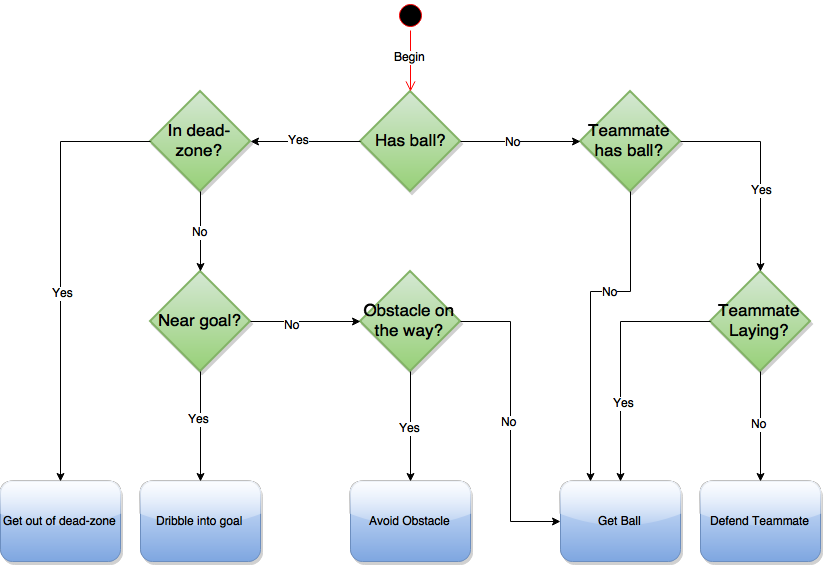
\includegraphics[width=\ScaleIfNeeded]{Grafiken/KI/attackerCenter_v2}
	\caption{Stürmer Entscheidungsbaum}
	\label{Stürmer Entscheidungsbaum}
\end{figure}

\subsection{Standardrolle: Verteidiger}
\begin{figure}[H]
	\centering
	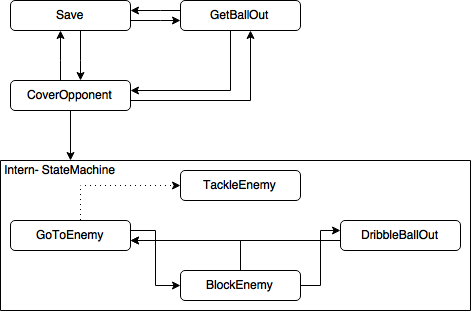
\includegraphics[width=\ScaleIfNeeded]{Grafiken/KI/defender/defender.png}
	\caption{State-Automat des Verteidigers}
	\label{State-Automat des Verteidigers}
\end{figure}
Das folgende Kapitel beschreibt die Funktionsweise und den Prozess zur Erstellung der Rolle des Verteidigers.

\subsubsection{Vorgehensweise}
\begin{figure}[H]
	\centering
	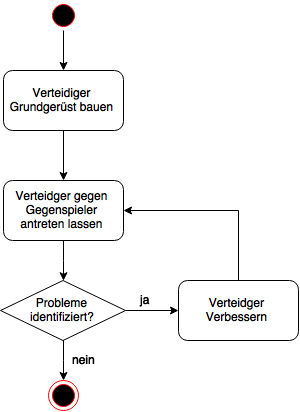
\includegraphics[width=\ScaleIfNeeded]{Grafiken/KI/defender/vorgehensweise.png}
	\caption{Vorgehensweise zur Entwicklung des Verteidigers}
	\label{Vorgehensweise-Verteidigers}
\end{figure}
Der in Abbildung \ref{Vorgehensweise-Verteidgers} dargestellte Prozess ist der Anforderung geschuldet zu einem m"oglichst fr"uhen Zeitpunkt bereits einen funktionierenden Spieler auf das Feld schicken zu k"onnen. Deswegen wurde ein iterativer Prozess gew"ahlt, dabei wird initial ein einfaches Grundger"ust entwickelt welches anschlie"senden Zyklisch verbessert werden kann. Der Prozess kann verlassen werden, wenn keine Zeit mehr f"ur Verbesserungen vorhanden ist, oder keine weiteren Probleme mit der Logik des Verteidigers gefunden werden k"onnen.\\
\\
\subsubsection{Use-Cases}
\begin{figure}[H]
	\centering
	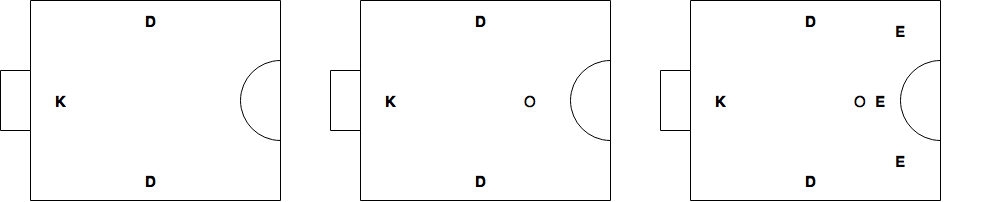
\includegraphics[width=\ScaleIfNeeded]{Grafiken/KI/defender/useCases.png}
	\caption{Die Use-Cases des Verteidigers}
	\label{Usecases-Verteidigers}
\end{figure}

F"ur den Verteidiger wurden die in Abbildung \ref{Usecases-Verteidigers} ermittelten Use-Cases definiert. Dabei gilt zu beachten, dass diese nicht den Anspruch haben alle m"oglichen F"alle abzubilden, sich aber auf einige wenige wichtige zu reduzieren. Dieses Vorgehen ist der Anforderung des einfachen Grundger"ustet geschuldet. F"uer die Use-Cases wurde ferner die idealisierende Annahme getroffen, dass auf der eigenen Spielfeldseite nur Verteidiger existieren. Ferner wurde dem gegnerischen Spieler eine h"ohere Priorit"at zugeteilt als dem Ball, die Annahme hierbei ist, dass der Ball durch den gegnerische Spieler in das Spielfeld getragen wird. Sollte der Ball frei sein und ein gegnerischer Spieler auf der eigenen Feldh"alfte sein, bewegt sich dieser auf den Ball zu, da er von dem Verteidiger gedeckt wird, sollten diese gleichzeitig bei dem Ball ankommen, die daraus resultierende Situation ist dann wieder der erst genannten gleich.

paragraph{UseCase: Spielgeschehen auf anderer Spielh"alfte}
Weder der Ball noch Gegnerische Spieler befinden sich auf der eigenen Spielh"alfte.
paragraph{UseCase: Ball in eigener Spielh"alfte}
Der Ball jedoch keine gegnerischen Spieler befinden sich auf der eigenen Spielh"alfte.
paragraph{UseCase: Gegner (mit Ball) in eigener Spielh"alfte}
Gegnerische Spieler befinden sich auf dem Spielfeld. Dabei ist es unerheblich ob der Ball ebenfalls mit auf dem Spielfeld ist.

%%%%%%%%%%%%%%%%%%%%%%%%%%%%%%%%%%%%%%%%%%%%%%%%%%%%%%%%%%%%%%%%%%%%%%%%%%%%%%%%%%%%%%%%%%
%%%%%%%%%%%%%%%%%%%%%%%%%%%%%%%%%%%%%%%%%%%%%%%%%%%%%%%%%%%%%%%%%%%%%%%%%%%%%%%%%%%%%%%%%%
%%%%%%%%%%%%%%%%%%%%%%%%%%%%%%%%%%%%%%%%%%%%%%%%%%%%%%%%%%%%%%%%%%%%%%%%%%%%%%%%%%%%%%%%%%

\subsection{Standardrolle: Mittelfeld}
\textit{Verfasser: Lohr}\\
\subsubsection{Planung, Evaluierung von Frameworks}
Zu Anfang wurde die Vorgehensweise geplant und verschiedene Frameworks evaluiert. Unter anderem wurden Zigorat und Delta3D, zwei Frameworks, welche in C++ geschrieben wurden, evaluiert. Zigorat war zu rudimentär, da wichtige Aktionen, z.B. Laufen, noch nicht implementiert waren. Delta3D war zu instabil. \par
Parallel dazu wurde recherchiert, wie eine KI am besten implementiert wird. Hierzu gibt es zwei Ansätze:
\begin{itemize}
 \item State-Driven Agent Design
 \item Goal-Driven Agent Design
\end{itemize}

\subsubsection{State-Driven Agent Design}
Das State-Driven Agent Design basiert auf Zustandsautomaten, wie sie auch in UML definiert wurden. Ein Zustandsautomat setzt sich zusammen auf verschiedenen Zuständen (States), davon genau ein Startzustand und min. ein Endzustand. Die Übergänge (Transitions) von einem Zustand in einen anderen werden durch Ereignisse (Events) ausgelöst.

\begin{figure}[ht]
	\centering
  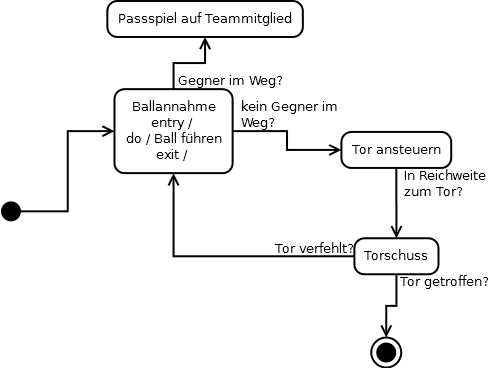
\includegraphics[width=0.85\textwidth]{Grafiken/KI/Bsp-Zustandsdiagramm.png}
	\caption{Ein stark vereinfachter Zustandsautomat}
	\label{fig1}
\end{figure}

Es gibt mehrere Möglichkeiten einen Zustandsautomaten zu implementieren. Es gibt unter anderem verschiedene Bibliotheken, die das implementieren eines Zustandsautomaten erleichtern. Unter anderem für C++: Boost.MSM (Meta State Machine), Boost.Statechart und Qt Statemachine Framework (aus dem Qt Framework). Für Java erschien die Tungsten FSM von Continuent am ausgereiftesten. Die Option ein auf Eclipse basierendes Tool namens Yakindu Statechart Tools\footnote{\url{http://statecharts.org/}} zu nutzen wurde verworfen, da nicht sicher war, wie sich das in den schon bestehenden Sourcecode einfügt.

\subsubsection{Goal-Driven Agent Design}
Das Goal-Driven Agent Design wird in \cite[S. 379 ff.]{buckland2005programming} beschrieben. Es besteht aus Zielen, die entweder weitere Unterziele beinhalten können, oder sie sind selber ein atomarer Bestandteil, und haben keine weiteren Unterziele mehr. (vgl. Kompositionsmuster \ref{fig2} aus \cite{gamma1994design}) Ob ein Ziel erreicht wurde, wird dadurch bestimmt, ob gewisse Unterziele erreicht wurden oder nicht. Schlägt ein Ziel fehl kann es neu ausgeführt werden.

\begin{figure}[ht]
	\centering
  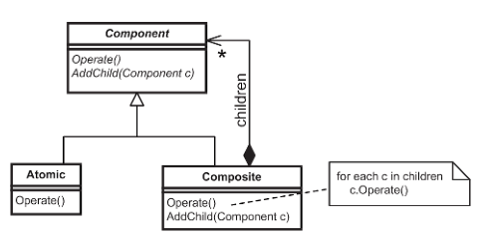
\includegraphics[width=0.85\textwidth]{Grafiken/KI/goal-driven.png}
	\caption{Das Kompositionsmuster. Grafik entstammt \cite[S. 383]{buckland2005programming}}
	\label{fig2}
\end{figure}

\subsubsection{Tungsten FSM}
Es wurde das Tungsten FSM von Continuent für eine Beispielimplementierung herangezogen. Die Tungsten FSM besteht unter anderem aus
\begin{itemize}
 \item States
 \item Transitions
 \item Actions
 \item Guards
\end{itemize}
Die Funktionsweise wurde im Wiki (Robofreunde n. V.) unter Tungsten\_FSM festgehalten. Die grundlegenden Funktionen seien hier nochmal wiederholt:

\paragraph{States}
Zustände werden wie folgt definiert:
\begin{lstlisting}
State haveBall = new State("Habe_Ball", StateType.START);
State gotoGoalWithBall = new State("Laufe_zu_Tor", StateType.ACTIVE);
State shootBallToGoal = new State("Torschuss", StateType.END);
\end{lstlisting}
Es gibt drei Arten von Zuständen:
\begin{itemize}
 \item \underline{Start}: Jede Statemachine hat genau einen Startzustand. Nach dem Start der Machine geht diese automatisch in diesen Zustand
 \item \underline{End}: Jede Statemachine braucht min. einen Endzustand. Dieser terminiert die Statemachine
 \item \underline{Active}: Jeder Zustand, der weder Start- noch Endzustand ist
\end{itemize}

\paragraph{Transitions}
Ein Zustandsübergang wird dadurch definiert von welchen Zustand aus er in welchen Zustand wechselt und unter welchen Umständen (Guard) und welche Aktion (Action) er dabei ausführt. In dem nächsten Beispiel sieht man einen Übergang von Zustand 1 in Zustand 2, falls ein Event vom Typ MeinEvent auftritt. Dabei wird die Action NullAction ausgeführt:
\begin{lstlisting}
Transition t = new Transition("Zustand1_zu_Zustand2", new EventTypeGuard(MeinEvent.class),
                    zustand1, new NullAction(), zustand2);
\end{lstlisting}

\paragraph{StateTransitionMap}
Alle Zustände und Zustandsübergänge werden in einer Map gespeichert:
\begin{lstlisting}
StateTransitionMap map = new StateTransitionMap();
map.addState(zustand1);
map.addState(zustand2);
map.addTransition(t);
\end{lstlisting}

\paragraph{Action}
Eine Action wird beim Übergang in einen anderen Zustand oder beim Eintritt oder Austritt aus einem Zustand ausgeführt. Das Interface Action ist zu implementieren, und eine Methode \underline{doAction} muss definiert werden:
\begin{lstlisting}
public class NullAction implements Action{
        @Override
        public void doAction(Event message, Entity entity, Transition transition, int actionType) 
        throws TransitionRollbackException, TransitionFailureException, InterruptedException
        {
            // Hier kommt die Logik hin
        }
    }
\end{lstlisting}

\paragraph{Guard}
Ein Guard überprüft, ob ein Zustandsübergang genommen wird, oder nicht. Ein Guard muss das Interface Guard implementieren und die Methode \underline{accept} definieren:
\begin{lstlisting}
public class OwnGuard implements Guard
{
    @Override
    public boolean accept(Event message, Entity entity, State state)
    {
        // Hier kommt die Logik hin
    }   
}
\end{lstlisting}
Es gibt bereits einige vordefinierten Guards, wie z.B. EventTypeGuard, der nur positiv wird, wenn ein bestimmter Zustand geworfen wird.

\subsubsection{Mittelfeldspieler}
Mit der Tungsten FSM wurde neben einem minimalen Bot auch ein Bot programmiert, der die Rolle ``Mittelfeldspieler'' einnehmen soll. Es wurden unter anderem folgende Use-Cases aufgestellt:

\begin{itemize}
 \item Eigene Mannschaft im Ballbesitz
 \begin{itemize}
  \item Solange die eigene Mannschaft im Ballbesitz ist, soll der Bot Abstand zum Ball halten
  \item Der Bot soll passiv bleiben, und versuchen das Vorankommen von gegnerischen Spieler zu verhindern
  \item Positionierung evtl. zwischen einem gegnerischen Spieler und dem ballbesitzendem eigenen Spieler um diesem einen, vom Gegner ungehinderten Lauf in Richtung Tor zu ermöglichen
 \end{itemize}
 
 \item Gegner im Ballbesitz
 \begin{itemize}
  \item Der Bot soll versuchen aktiv dem Gegner den Ball abzunehmen
  \item keine Behinderung von eigenen Mitspielern
 \end{itemize}
 
 \item Eigener Spieler im Ballbesitz
 \begin{itemize}
  \item Falls keine Behinderung durch gegnerische Spieler: Versuche selber Tor zu schießen
  \item Falls der Spieler bedrängt wird, nach Möglichkeit auf freistehenden Mitspieler passe
 \end{itemize}
\end{itemize}
Die Anwendungsfälle (Use cases) wurden anschaulich dargestellt (siehe Anhang \ref{usecases_midfielder}), und aus diesen Use Cases leitet sich das Zustandsdiagramm ab, nach dem der Bot agiert. Das Zustandsdiagramm befindet sich in Anhang \ref{statechart_midfielder}

%%%%%%%%%%%%%%%%%%%%%%%%%%%%%%%%%%%%%%%%%%%%%%%%%%%%%%%%%%%%%%%%%%%%%%%%%%%%%%%%%%%%%%%%%%
%%%%%%%%%%%%%%%%%%%%%%%%%%%%%%%%%%%%%%%%%%%%%%%%%%%%%%%%%%%%%%%%%%%%%%%%%%%%%%%%%%%%%%%%%%
%%%%%%%%%%%%%%%%%%%%%%%%%%%%%%%%%%%%%%%%%%%%%%%%%%%%%%%%%%%%%%%%%%%%%%%%%%%%%%%%%%%%%%%%%%
\subsection{Spezialrollen: Standardsituationen}
\textit{Verfasser: Stumpf}\\
\\
Die Standardsituationen sind über Spezialrollen umgesetzt. Die aktuelle Strategie weist -- falls das Spiel in einer Standardsituation ist -- einem der Spieler die Spezialrolle zu, mit dieser umzugehen.\\
\\
Die verschiedenen Spezialrollen für Standards werden hier kurz vorgestellt. Die folgenden Statemachines sollen einen Überblick über die benötigte Funktionalität geben.\\
\\
Sie befinden sich im Package\\\texttt{magma.agent.decision.simple.robofreunde.role.standard\_situations}.

\subsubsection{Ansto{\ss}}
\textit{Verfasser: Stumpf}\\
\\
\begin{figure}[H]
	\centering
	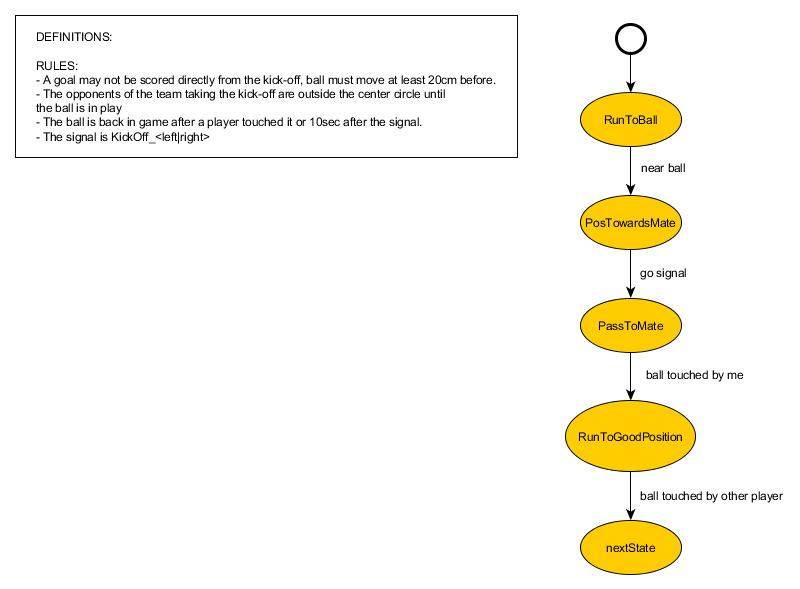
\includegraphics[width=\textwidth]{Grafiken/KI/Standardsituationen/KickoffSM}
	\caption{Spezialrolle - Kickoff}
	\label{fig:Standard - Kickoff}
\end{figure}

Der Ansto{\ss} besteht generell aus einer Positionierung am Ball mit anschließendem Pass. Es ist darauf zu achten die Spielregel für den Ansto{\ss} nicht zu verletzen. Nachdem der Ball berührt wurde, darf der gleiche Spieler diesen nicht erneut berühren. Deshalb wird hier nach dem Pass eine Neupositionierung vorgenommen und somit versucht dem Ball aus dem Weg zu gehen.\\
\\
Benötigte Behaviors sind KickToPosition und RunToPosition. Eine Logik für die Positionierung am Ball muss ebenso wie die Neupositionierung vorhanden sein.\\
\\
Es wurde hier der Pass gewählt, da der uns zur Verfügung stehende Kick leider nicht weit genug kommt, als dass sich ein Kick in die gegnerische Hälfte lohnen würde.

\subsubsection{Freisto{\ss}, Ecke}
\textit{Verfasser: Stumpf}\\
\\
\begin{figure}[H]
	\centering
	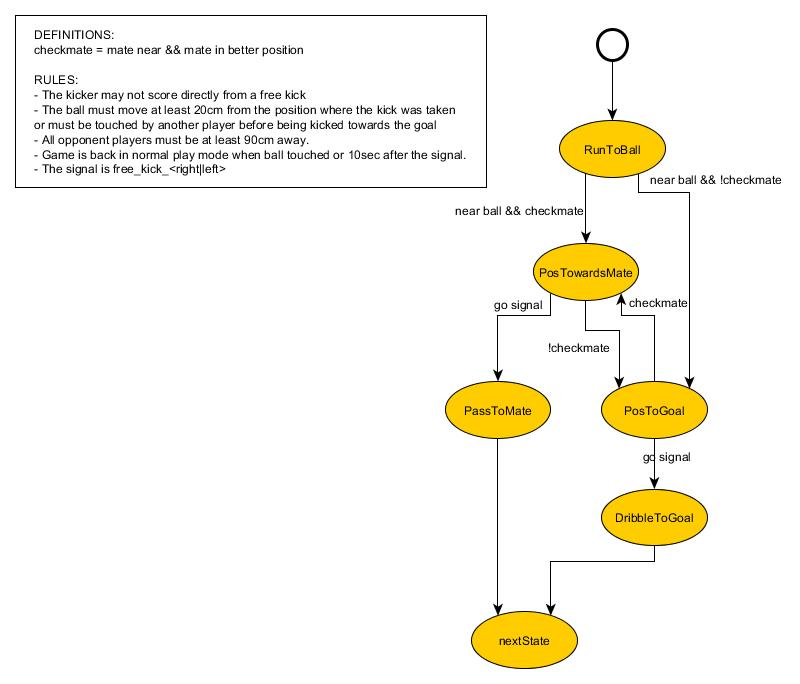
\includegraphics[width=\textwidth]{Grafiken/KI/Standardsituationen/FreeKickSM}
	\caption{Spezialrolle - Freekick}
	\label{fig:Standard - Freekick, Cornerkick}
\end{figure}

Vorweg zu erwähnen ist, dass der Freisto{\ss} aus dem aktuellen Regelwerk (Stand: 2015) entfernt und durch Auszeiten ersetzt wurde. Insofern ist diese Implementierung nur der Vollständigkeit und Kompatibilität halber aufgeführt.\\
\\
Da beim Freisto{\ss} kein direktes Tor erzielt werden darf wird hier einfach zum nächsten Mitspieler in der Nähe gepasst, sollte kein Mitspieler in der Nähe sein, der in einer besseren Position als man selbst ist, so wird in Richtung Tor gedribbelt.\\
\\
Benötigte Behaviors sind KickToPosition, RunToPosition sowie DribbleBall. Es wird eine Logik für die Positionierung vorausgesetzt.\\
\\
Als Zustandsautomat für die Standardsituation Ecke wurde der selbe verwendet wie für den Freisto{\ss}.

\subsubsection{Einwurf}
\textit{Verfasser: Stumpf}\\
\\
\begin{figure}[H]
	\centering
	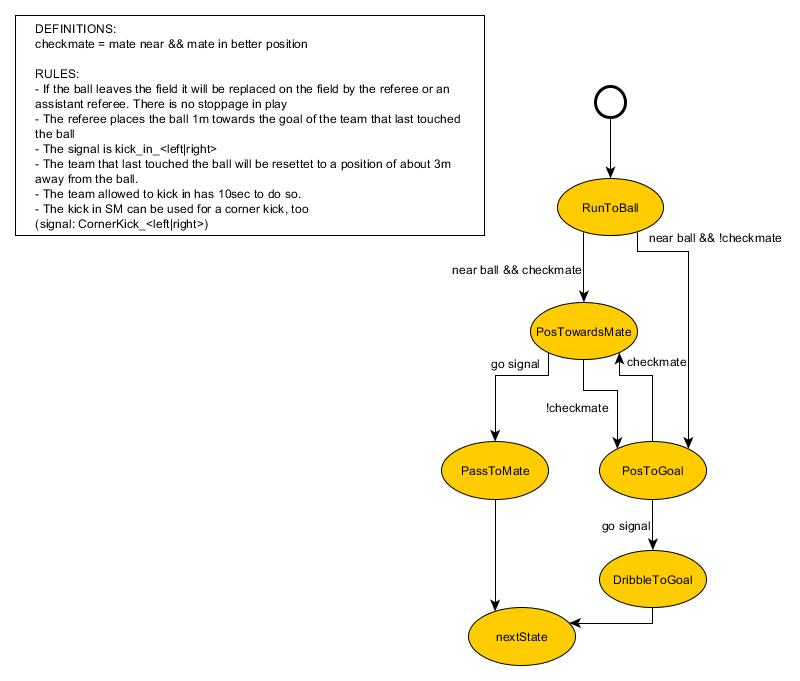
\includegraphics[width=\textwidth]{Grafiken/KI/Standardsituationen/KickInSM}
	\caption{Spezialrolle - Kick in}
	\label{fig:Standard - KickIn}
\end{figure}

Der Zustandsautomat des Einwurfs ist grundsätzlich gleich dem des Freisto{\ss}es, da nicht geworfen, sondern gekickt wird.

\subsubsection{Absto{\ss}}
\textit{Verfasser: Stumpf}\\
\\
\begin{figure}[H]
	\centering
	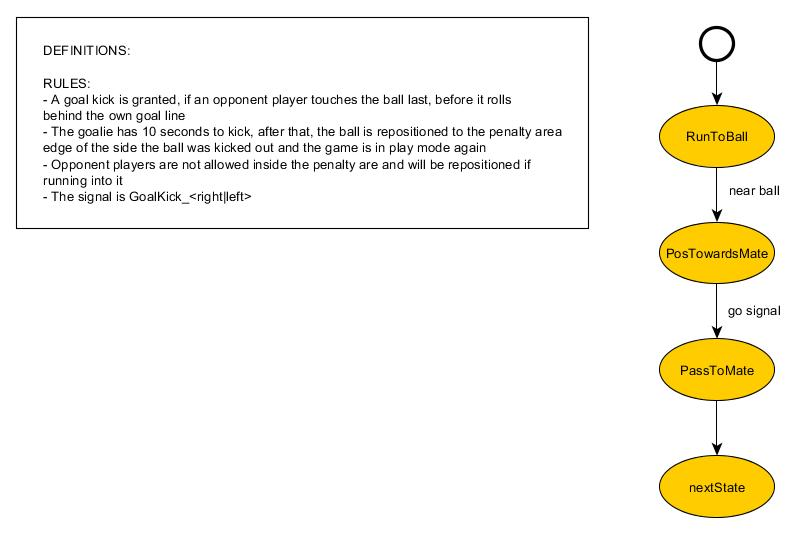
\includegraphics[width=\textwidth]{Grafiken/KI/Standardsituationen/GoalKickSM}
	\caption{Spezialrolle - Goalkick}
	\label{fig:Standard - Goalkick}
\end{figure}

Der Zustandsautomat des Absto{\ss}es ist grundsätzlich gleich dem des Ansto{\ss}es. Der einzige Unterschied ist, dass der Ball nach einem Abstoß erneut berührt werden darf, weshalb die Neupositionierung und Vermeidung der Ballberührung wegfällt.

\subsubsection{Implementierung}
\textit{Verfasser: Stumpf}\\
\\
Bei der Implementierung der Standardsituationen wollte ich unnötige Redundanz vermeiden. Die Rollen waren sich so ähnlich, dass ich mich entschlossen habe, sie auf gemeinsamen States aufzubauen.\\
\\
Die beiden gemeinsam verwendeten States sind InteractWithBall und MoveToBall.\\
\\
Solange man sich nicht in der Nähe des Balles befindet wird man sich im State \textbf{MoveToBall} aufhalten. Dieser State gibt intern eine RunToPosition Behavior zurück, mit dem Ziel sich in die Nähe des Balls zu begeben.\\
\\
Ist man in der Nähe des Balls, so wird man in den \textbf{InteractWithBall} State wechseln. Dieser enthält die meiste Logik und entscheidet wie mit dem Ball interagiert werden soll.\\ 
Intern wird zuerst entschieden, welche Interaktion ausgeführt werden soll. Zur Auswahl stehen:
\begin{itemize}
\item Zum Tor Dribblen
\item Zum Tor Schießen
\item Zu Mitspieler passen
\end{itemize}
Die Interaktionen sind über eine Methode des States \\
\\
\texttt{public void setActiveInteractions(\\boolean dribbleToGoal, boolean passToMate, boolean kickToGoal)}\\
\\
konfigurierbar. Es wird nur aus aktiven Interaktionen ausgewählt.
Die Entscheidung wird getroffen anhand von gemeinsamer Logik, zum Beispiel \textit{\glqq Befinde ich mich in der Nähe des Tors, so dass ein Torschuss erfolgreich sein könnte?\grqq}, oder \textit{\glqq Ist ein Mitspieler in der Nähe, der besser steht als ich?\grqq}.

\section{Grafisches Debugging}\label{se:Grafisches Debugging}
\textbf{-> TODO: Felix}
\section{Strategien}
\textbf{-> TODO: Freddy}
\section{Strategie-Entscheider}
\textbf{-> TODO: Freddy}
\section{Zusammenfassung und Ausblick}
\textbf{-> TODO: Freddy}
\textit{Ergebnisse und Vermächtnis...}

\section{Verzeichnisse}
\listoffigures

\lstlistoflistings

\begin{appendices}
\section{Use cases für den Bot ``Mittelfeldspieler''}
\label{usecases_midfielder}

\noindent\makebox[\textwidth]{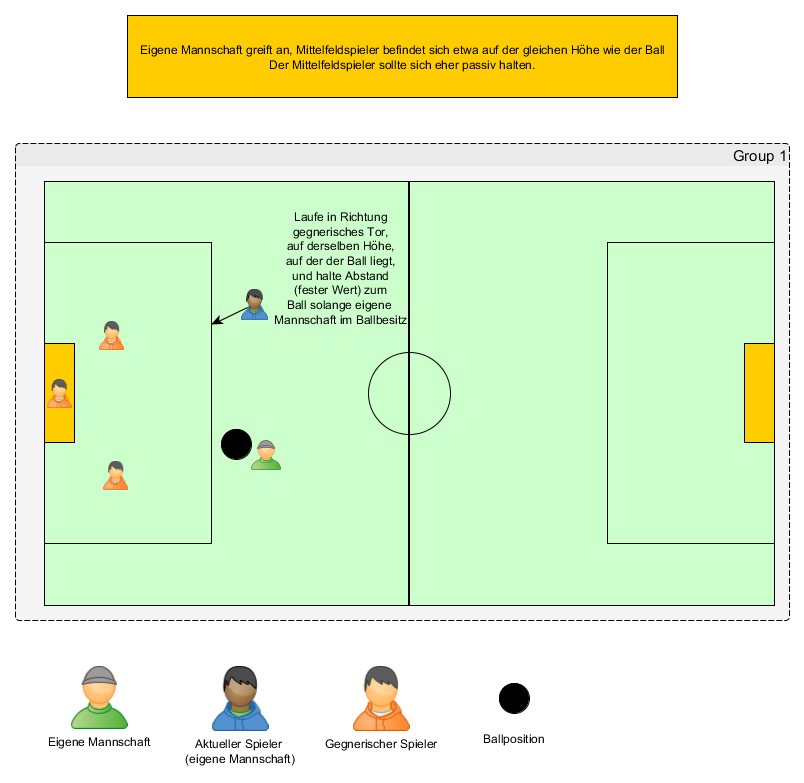
\includegraphics[angle=90,origin=c,width=0.9\paperwidth]{Grafiken/KI/mittelfeldspieler/eigene_mannschaft_im_angriff.png}}

\noindent\makebox[\textwidth]{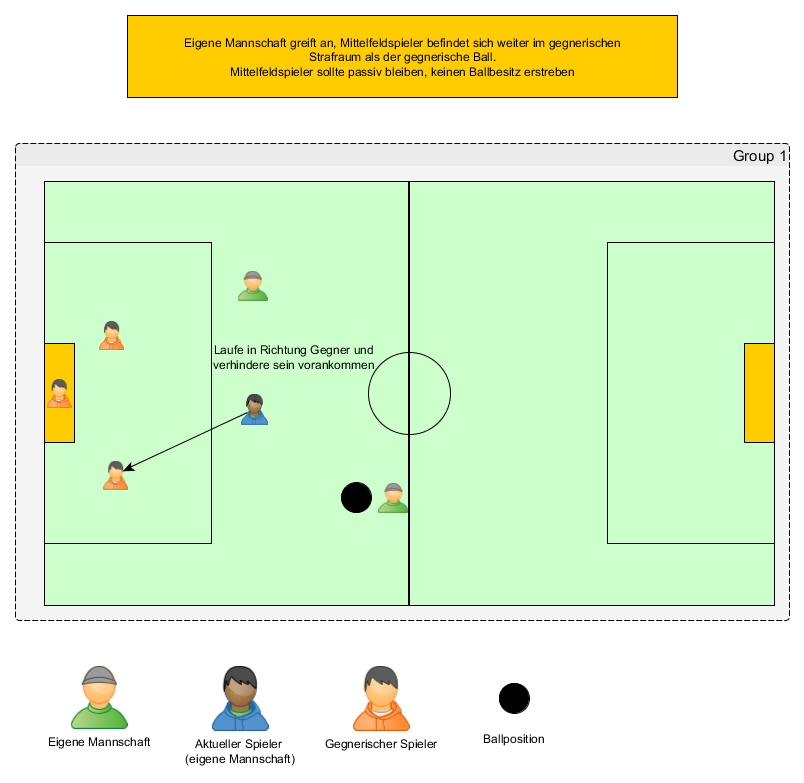
\includegraphics[angle=90,origin=c,width=0.9\paperwidth]{Grafiken/KI/mittelfeldspieler/eigene_mannschaft_im_angriff_fall_2.png}}

\noindent\makebox[\textwidth]{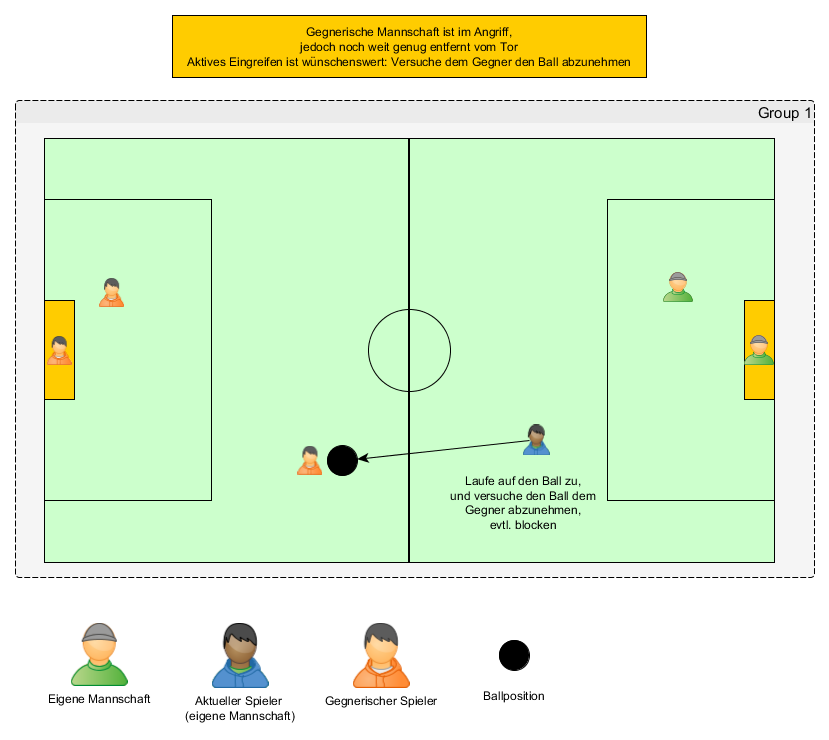
\includegraphics[angle=90,origin=c,width=0.9\paperwidth]{Grafiken/KI/mittelfeldspieler/gegnerische_mannschaft_im_angriff.png}}

\noindent\makebox[\textwidth]{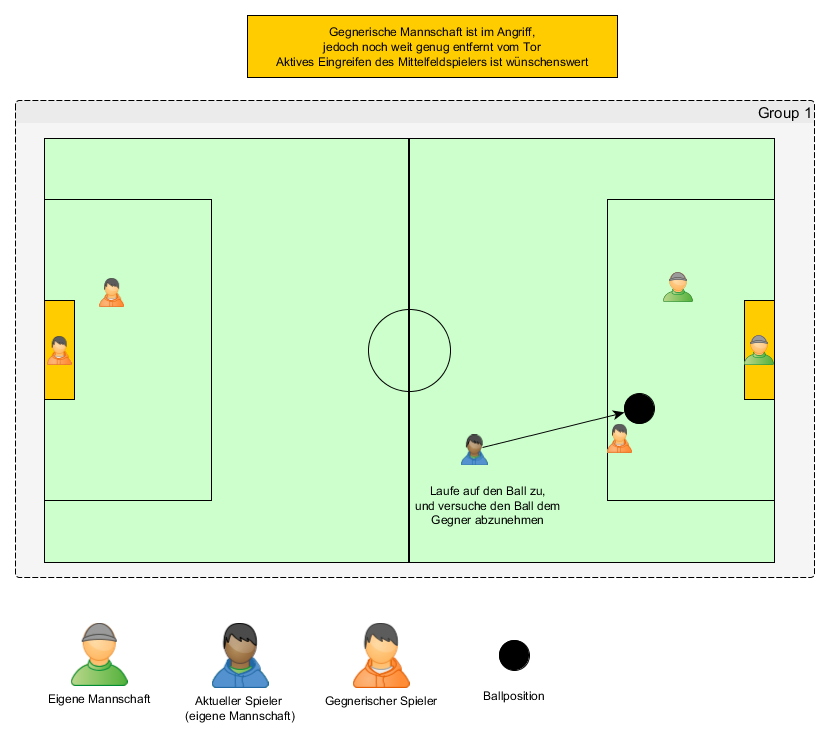
\includegraphics[angle=90,origin=c,width=0.9\paperwidth]{Grafiken/KI/mittelfeldspieler/gegnerische_mannschaft_im_angriff_fall_2.png}}

\section{Zustandsdiagramm für den Bot ``Mittelfeldspieler''}
\label{statechart_midfielder}

\noindent\makebox[\textwidth]{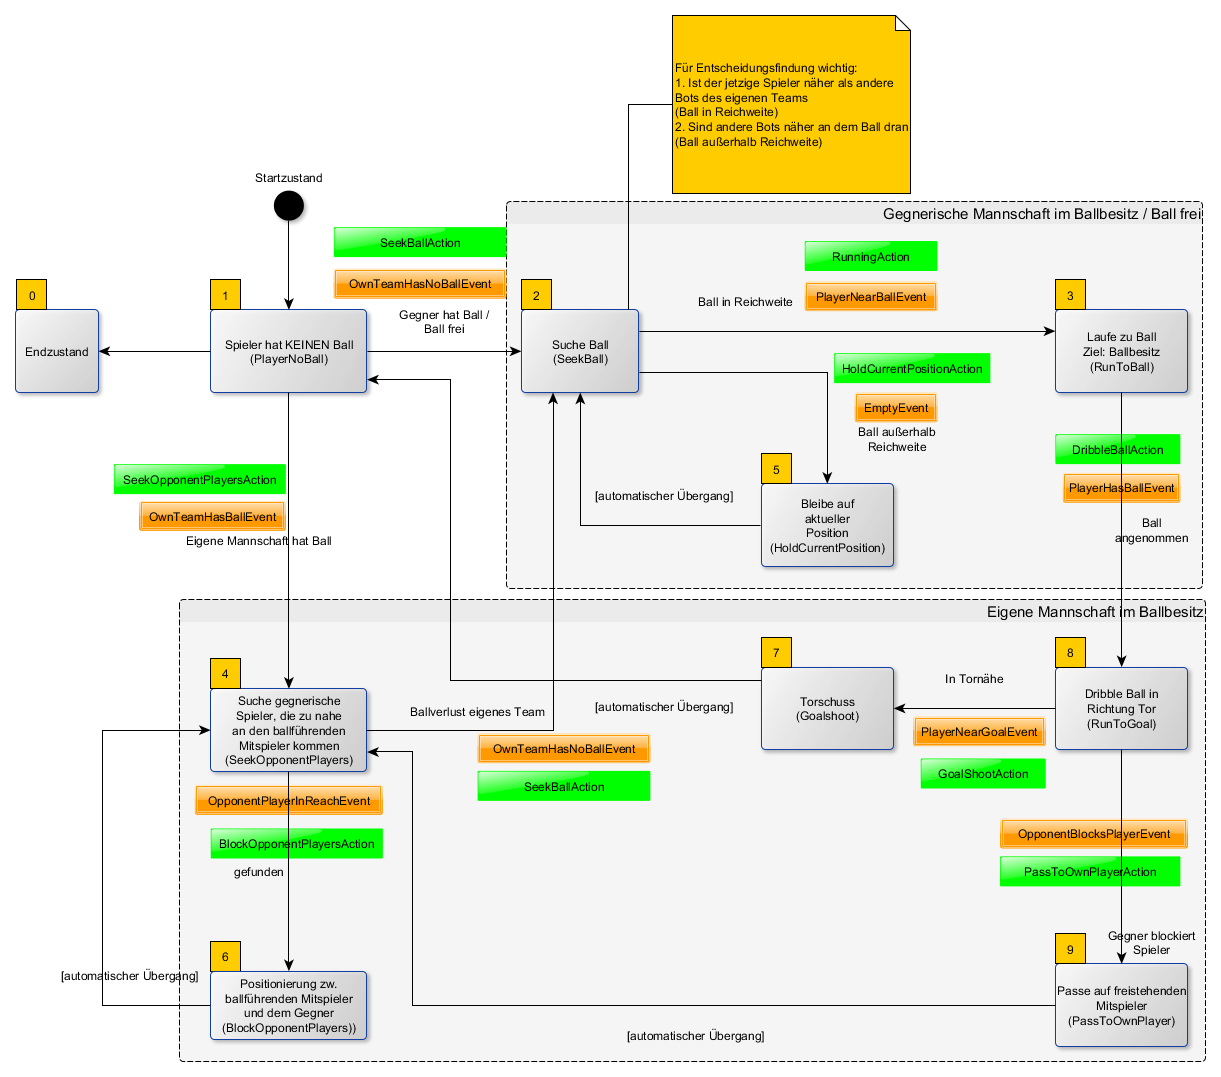
\includegraphics[angle=90,origin=c,width=0.9\paperwidth]{Grafiken/KI/mittelfeldspieler/mittelfeldspieler.png}}

\end{appendices}

\end{document}